%# -*- coding: utf-8-unix -*-
%%==================================================
%% thesis.tex
%%==================================================

% 双面打印
%\documentclass[doctor, openright, twoside]{sjtuthesis}
\documentclass[bachelor, fontset=fandol,  openany, twoside, submit]{sjtuthesis}
% \documentclass[master, review]{sjtuthesis}
% \documentclass[%
%   bachelor|master|doctor,	% 必选项
%   fontset=fandol|windows|mac|ubuntu|adobe|founder, % 字体选项
%   oneside|twoside,		% 单面打印,双面打印(奇偶页交换页边距,默认)
%   openany|openright, 		% 可以在奇数或者偶数页开新章|只在奇数页开新章(默认)
%   english,			% 启用英文模版
%   review,	 		% 盲审论文,隐去作者姓名、学号、导师姓名、致谢、发表论文和参与的项目
%   submit			% 定稿提交的论文,插入签名扫描版的原创性声明、授权声明 
% ]

% 逐个导入参考文献数据库
\addbibresource{bib/spamming.bib}
% \addbibresource{bib/chap2.bib}

\usepackage[linesnumbered, boxed, ruled, commentsnumbered,algo2e]{algorithm2e}

\CTEXsetup[format+={\heiti}]{chapter}
\CTEXsetup[indent={2em}, format+={\heiti}]{subsection}
\CTEXsetup[indent={2em}, format+={\heiti}]{section}

\begin{document}

%% 无编号内容:中英文论文封面、授权页
%# -*- coding: utf-8-unix -*-
\title{网络人工水军检测研究}
\author{金瑞东}
\advisor{阮娜}
% \coadvisor{某某教授}
\defenddate{2018年5月8日}
\school{上海交通大学}
\institute{电子信息与电气工程学院}
\studentnumber{5140309334}
\major{计算机科学与技术}

\englishtitle{Research of Manual Spamming Detection}
\englishauthor{\textsc{Mo Mo}}
\englishadvisor{Prof. \textsc{Mou Mou}}
% \englishcoadvisor{Prof. \textsc{Uom Uom}}
\englishschool{Shanghai Jiao Tong University}
\englishinstitute{\textsc{Depart of XXX, School of XXX} \\
  \textsc{Shanghai Jiao Tong University} \\
  \textsc{Shanghai, P.R.China}}
\englishmajor{A Very Important Major}
\englishdate{Dec. 17th, 2014}


\maketitle

\makeatletter
%\ifsjtu@submit\relax
%	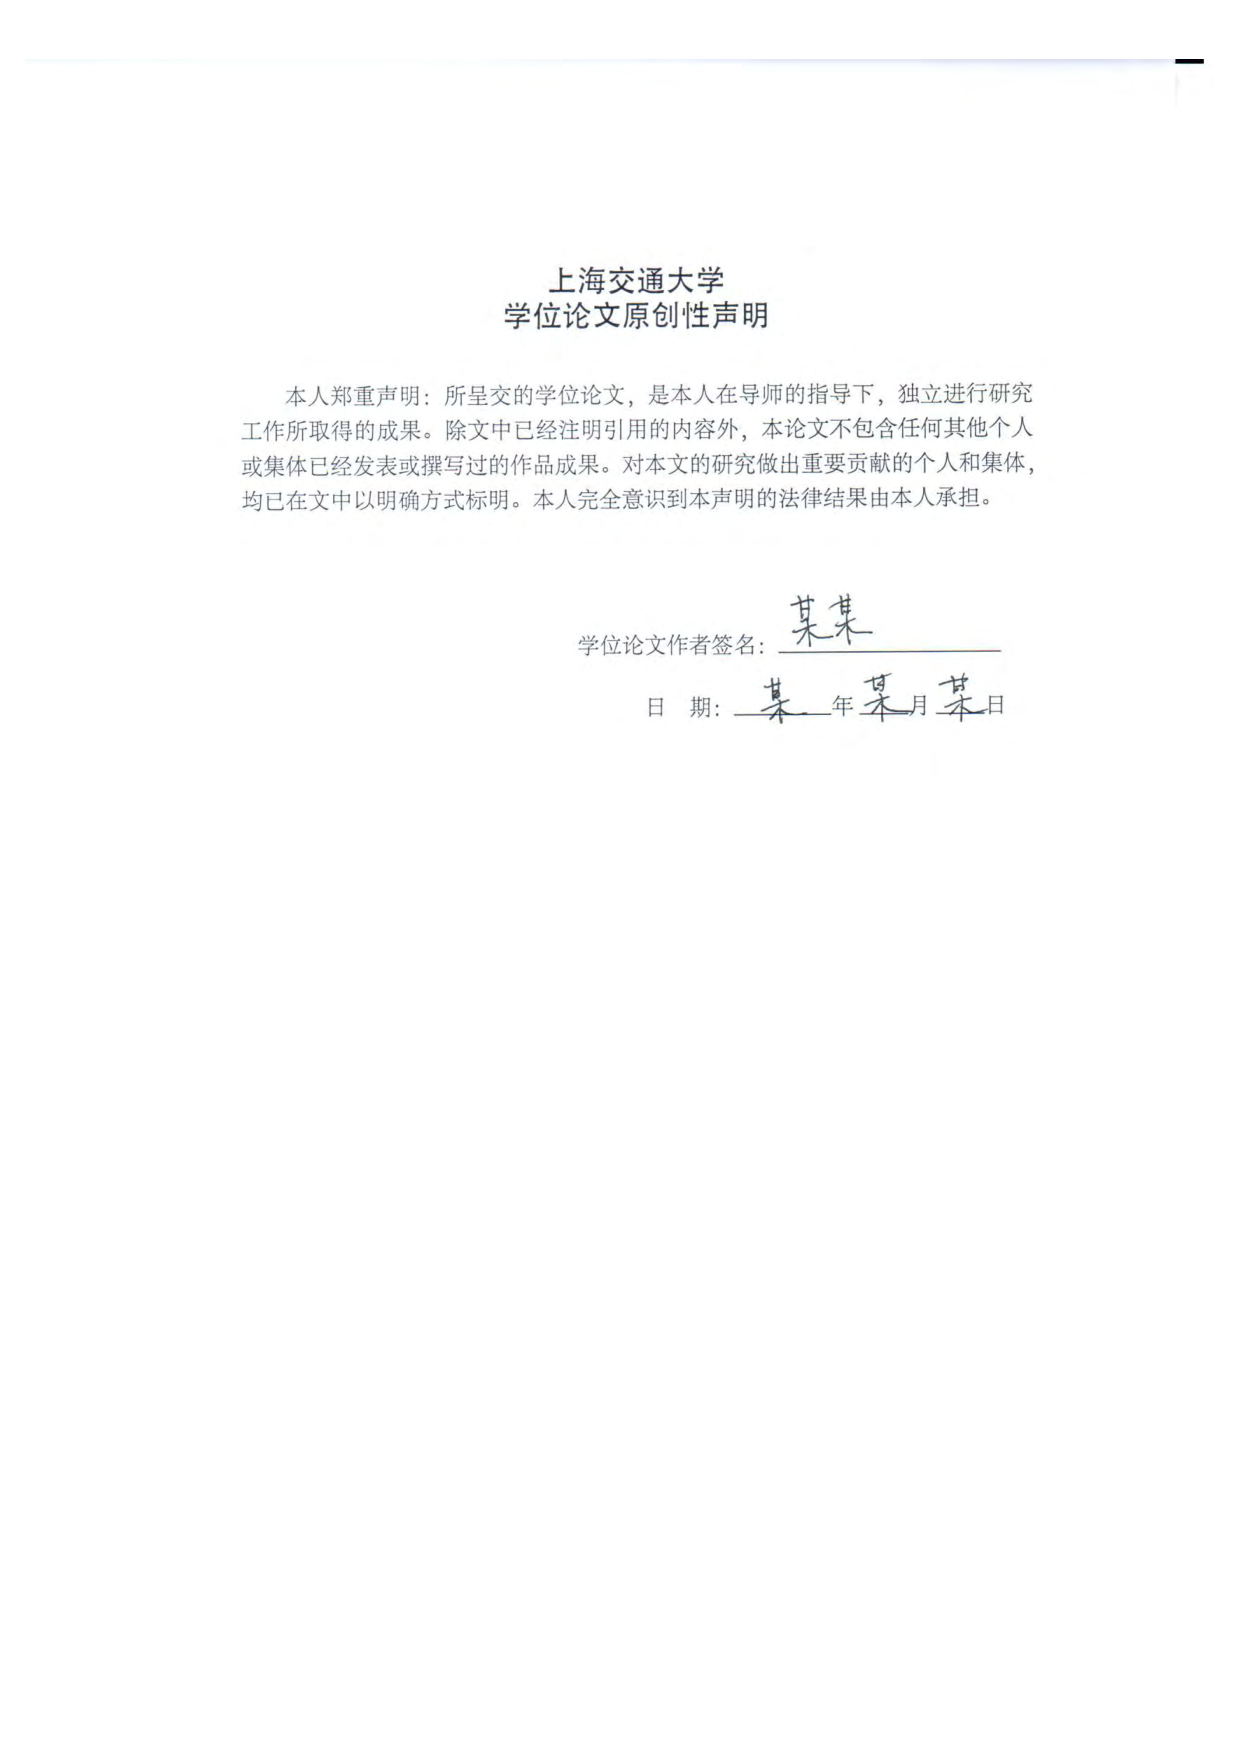
\includepdf{pdf/original.pdf}
%	\cleardoublepage
%	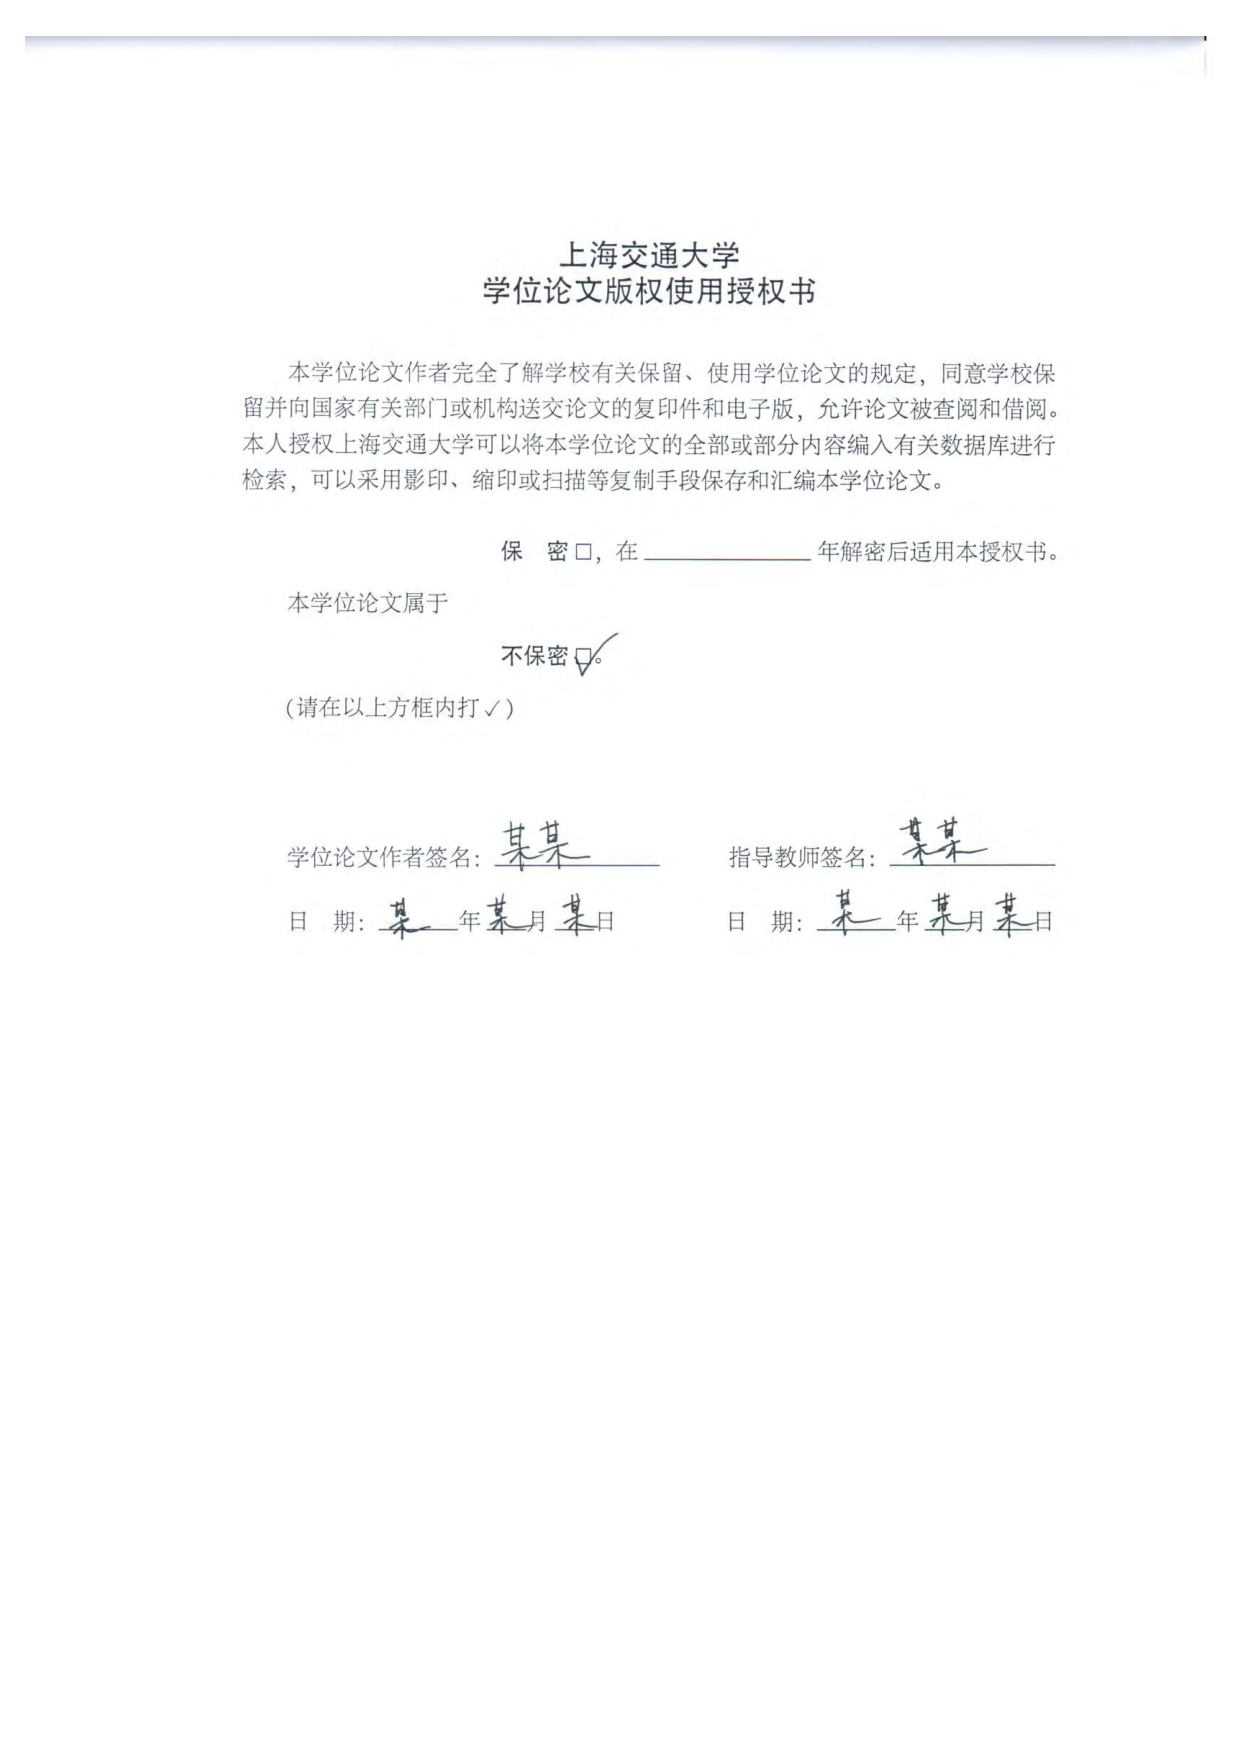
\includepdf{pdf/authorization.pdf}
%	\cleardoublepage
%\else
%\ifsjtu@review\relax
%exclude the original claim and authorization
%\else
%	\makeDeclareOriginal
%	\makeDeclareAuthorization
%\fi
%\fi
\makeatother


\frontmatter 	% 使用罗马数字对前言编号

%% 摘要
\pagestyle{main}
%# -*- coding: utf-8-unix -*-
%%==================================================
%% abstract.tex for SJTU Master Thesis
%%==================================================

\begin{abstract}

近年来,O2O(Online To Offline)电子商务平台在居民的消费生活中作用越来越重要。然而,在名誉和利益的驱动下,有一部分人试图使用网络诈骗的方式,例如发布水军评论和虚假内容,恶意操作线上市场。这种行为极大地危害了线上市场的环境,应当被立即侦测并驱除。而且,比起简单的僵尸网络机器水军,那些人工水军的隐蔽性和危害性更大。目前在网络水军检测领域已经存在各种成熟的方法。这些方法利用水军的爆发式活动特征和账户信息等特征进行机器学习,识别出水军用户。但是随着水军技术的不断革新,水军们已经掌握了躲避传统机器学习检测的方法,他们会控制水军活动的速率,并模仿正常用户的样子完善账户信息,传统的水军检测系统使用的算法和特征面临着效率不足的问题,我们急需找到与之前的水军检测原理相异的,高效的新特征和新方法。我们的调查显示地理位置因素可以很好地反映水军用户和普通用户之间的差异。在这篇论文中,我们分析了评论中店铺的地理位置,找到了水军用户和普通用户中地理位置特征分布的差异,并提出了一个基于隐马尔可夫模型的\emph{SpamTracer}模型用于分辨水军用户和正常用户。我们的实验结果展示了SpamTracer可以在不平衡的数据集中达到71\%的准确率(Accuracy)和76\%的召回率(Recall)。这个测试结果在稳定性上可以超过一些优秀的经典方法。此外,SpamTracer可以帮助我们分析人工水军的行动规律。这些规律反映了商家们倾向于在合适何地雇佣人工水军来增加收入。我们还发现了一小部分人工水军倾向于和在一个小商圈内的多个商家达成合作关系。

\keywords{\large O2O电子商务平台, 水军检测, 地理位置, 隐马尔可夫模型}
\end{abstract}

\begin{englishabstract}

Nowadays, O2O(Online To Offline) commercial platforms are playing a crucial role in our daily purchases. However, some people are trying to manipulate the online market maliciously by opinion spamming, a kind of web fraud behavior like writing fake reviews, due to fame and profits, which will harm online purchasing environment and should be detected and eliminated. Moreover, manual spammers are more deceptive compared with old web spambots. Several sophisticated and efficient methods have been proposed in spamming review detection field. Those methods apply spamming burst features and account characteristics to machine learning algorithms, and identify the spammers. However, with the evolution of spamming approaches, spammers can get away from detection systems. They can control the rate of spamming actions, and disguise as normal accounts. Thus current detection systems and features are facing with low efficiency. It's essential to find new efficient features and algorithms. Our investigation presented that geolocation can well reflect the distinctions between spammers and normal users. In this research, we analyzed the geolocations of shops in review, found the distinct distribution features of those in spamming and non-spamming users, and proposed a \emph{SpamTracer} model that can identify spammers and non-spammers by exploiting an improved HMM(Hidden Markov Model). Our experiment demonstrated that SpamTracer could achieve 71\% accuracy and 76\% recall in the unbalanced dataset, outperforming some excellent classical approaches in the aspect of stability. Furthermore, SpamTracer can help to analyze the regularities of spamming actions. Those regularities reflect the time and location in which online shops are likely to hire spammers to increase their turnover. We also found that a small group of spammers tend to work with plural shops located in a small business zone.

\englishkeywords{\large O2O Commercial Platform, Spamming Detection, Geolocation, Hidden Markov Model}
\end{englishabstract}



%% 目录、插图目录、表格目录
\tableofcontents
\listoffigures
\addcontentsline{toc}{chapter}{\listfigurename} %将插图目录加入全文目录
\listoftables
\addcontentsline{toc}{chapter}{\listtablename}  %将表格目录加入全文目录
\listofalgorithms
\addcontentsline{toc}{chapter}{\listalgorithmname} %将算法目录加入全文目录

%# -*- coding: utf-8-unix -*-
\begin{nomenclaturename}
\label{chap:symb}

\begin{longtable}{rl}
$x_i$ &  用户的评论中第$i$个评论的店铺的位置\\
$C$ &  用户的活跃区域的地理位置中心\\
$Distance(A, B)$ & 位置$A$和位置$B$的间隔距离 \\
$\gamma_{x_i}$ &  $x_i$的半径特征,即$x_i$和$C$的间隔距离\\
$f(x;\mu,\sigma)$ & 参数为$\mu$和$\sigma$的高斯分布\\
$N(\mu, \sigma^2)$ & 参数为$\mu$和$\sigma$的高斯分布 \\
$L$ &  标签变量\\
$\lambda$ = \{$\mathbf{A}$, $\mathbf{B}$, $\mathbf{\pi}$\} &  隐马尔可夫模型(HMM)\\
$\mathbf{A}$ &  HMM的转移概率 \\
$\mathbf{B}$ &  HMM的输出概率 \\
$\mathbf{\pi}$ &  HMM的初始化概率\\
$X_i$ &  第$i$个观测态变量\\
$X_{1:T}$ &  从$X_1$到$X_T$的观测态序列 \\
$P$ & 概率 \\
$Y_i$ &  第$i$个隐藏态变量\\
$Y_{1:T}$ &  从$Y_1$到$Y_T$的观测态序列 \\
$a_{j,k}$ &  转移概率$\mathbf{A}$的矩阵元素 \\
$b_j()$ &  输出概率$\mathbf{B}$的分布函数 \\
$\mathbf{M}$ &  店铺数据集\\
$\mathbf{R}$ &  用户数据集\\
\end{longtable}

\end{nomenclaturename}
 % 主要符号、缩略词对照表

\mainmatter	% 使用阿拉伯数字对正文编号

%% 正文内容
\pagestyle{main}
%# -*- coding: utf-8-unix -*-
%%==================================================
%% chapter01.tex for SJTU Master Thesis
%%==================================================

%\bibliographystyle{sjtu2}%[此处用于每章都生产参考文献]
\chapter{绪论}
\label{chap:intro}

\section{水军问题相关现状}

近年来随着信息网络和智能便携设备高速发展,人们的网络生活变化日新月异。与此同时,人们的衣食住行也和网络不断产生着联系。一方面,由于网络消费方便快捷,社交网络信息传播速度快的特点,越来越多的人选择通过网络进行社交和消费行为。中国互联网络信息中心发布的第41次《中国互联网络发展状况统计报告》显示:截止2017年12月,中国网民规模达7.72亿,其中手机上网人数占比达97.5\%;移动支付规模持续扩大,网民在线下消费使用手机网上支付比例由2016年底的50.3\%提升至65.5\%;电子商务持续快速增长,2017年1月至11月电子商务平台收入2188亿元,同比增长高达43.4\%。在世界范围内,2018年We Are Social和Hootsuite的最新全球数字报告显示,世界网民规模达到了40亿,其中使用智能手机上网的人数占比达52\%;Statista最新数据显示,2017年的电商市场年度总支出达到了近1.5万亿美元。全球范围内,使用电商平台购买商品(如衣服、食品、电子产品和玩具)的人数增长了8%,全球近18亿人在网上购物,占所有互联网用户的45%左右。另一方面,各种网络平台也在飞速发展。在中国范围内,淘宝\footnote{www.taobao.com}是深受欢迎的网购零售平台,拥有近5亿的注册用户数,每天有超过6000万的固定访客,同时每天的在线商品数已经超过了8亿件,平均每分钟售出4.8万件商品;大众点评\footnote{www.dianping.com}是一家独立第三方消费点评网站。大众点评不仅为用户提供商户信息、消费点评及消费优惠等信息服务,同时亦提供团购、餐厅预订、外卖及电子会员卡等线上到线下交易服务;微博\footnote{www.weibo.com}是中国广受欢迎的社交网络平台,是一个基于用户关系信息分享、传播以及获取的平台。用户可以用140字的文字更新信息,并实现即时分享。而在世界范围内,亚马逊\footnote{www.amazon.com}是网络上最早开始经营电子商务的公司之一,现在已成为全球商品品种最多的网上零售商和全球第二大互联网企业;Yelp\footnote{www.yelp.com}是发源于美国,现世界最著名的商户点评网站,囊括各地餐馆、购物中心、酒店、旅游等领域的商户;而Facebook\footnote{www.facebook.com}稳座世界范围社交网络头把交椅,拥有近20亿活跃使用者。可以说,网络消费平台和社交网络平台对人们的日常生活有着十分重要的作用。

\begin{figure}[htp]
	\centering
	\subcaptionbox{“紫光阁地沟油”事件\label{figure:spam-a}} %标题的长度,超过则会换行,如下一个小图。
	{
\includegraphics[height=9cm]{intro-2.jpg}}
	\hspace{4em}
	\subcaptionbox{微博水军刷转发量\label{figure:spam-b}}
	{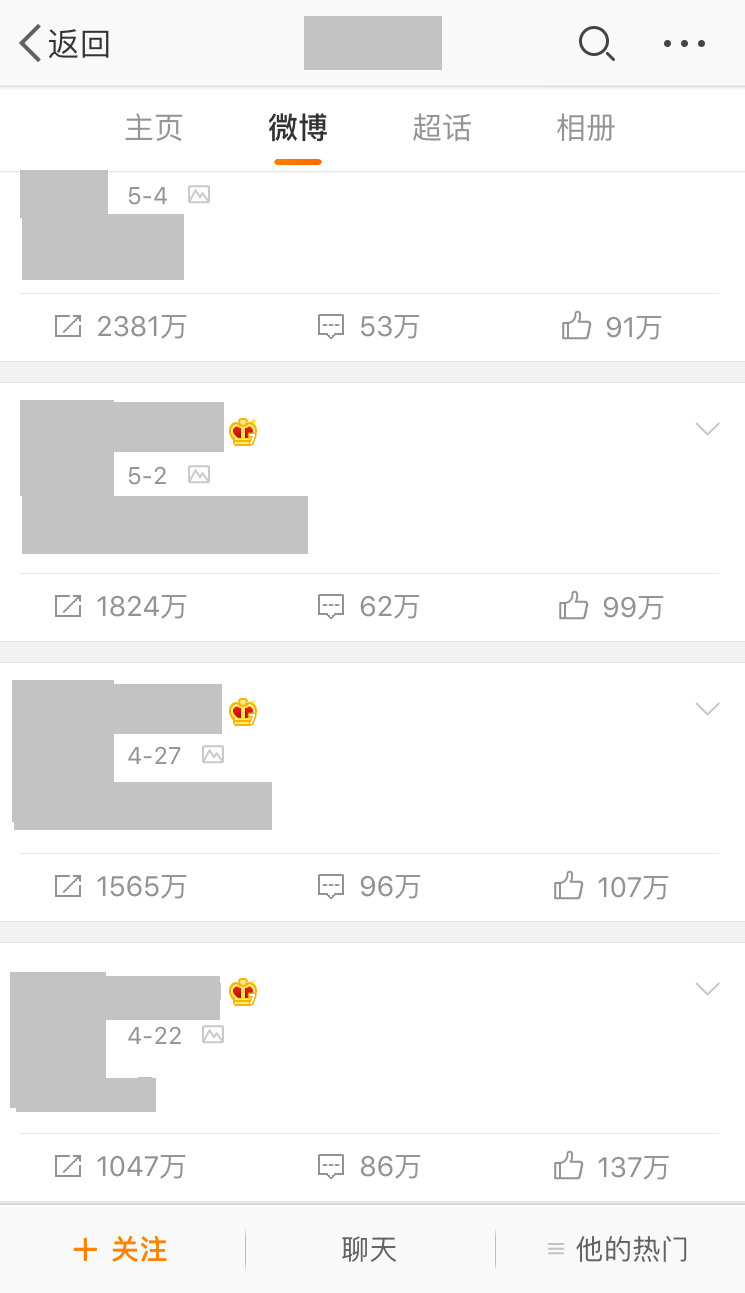
\includegraphics[height=9cm]{intro-3.png}}
	\caption[网络水军的表现]{网络水军的表现}
\end{figure}

但是,在利益的驱使下,如此庞大的市场中必然会出现秩序的破坏者。这些破坏者就是水军。他们依靠控制的大量账号,在社交网络中为雇主造势,在网购平台中恶意刷单,在评论网站中发布虚假的点评内容,以满足雇主的需求并获得利益。普通的网民在从众心理的诱导下,很容易被水军发布的言论所误导,对社交网络中的热点话题产生误解,或者在网络消费过程中蒙受经济损失。网络水军们甚至形成了成熟的黑色产业链:微博买粉丝买热搜,淘宝恶意刷单,大众点评刷好评,微信公众号刷流量等。低价雇佣真实用户进行水军行为的广告网络上也随处可见。水军的存在对当前的网络环境造成了恶劣的影响,是伴随着时代进步产生的新问题。水军们可以颠倒黑白将国家党建宣传机关说成卖地沟油的黑心饭店(如图~\ref{figure:spam-a}),也可以帮雇主疯狂地刷转发量(如图~\ref{figure:spam-b})。可以预见近期内,水军的检测在世界范围内都将是一项挑战。


尽管水军检测相关的研究已经进行了很多年,并且在NLP(Natural Language Processing)领域是一个老生常谈的问题,但是从安全和隐私角度来考虑的话,水军检测问题还有很多未经发掘的地方。伴随着机器学习和人工智能近年来的高速发展,机器学习+安全的新思维可以带给我们更多解决问题的思路。表~\ref{tbl:intro-1}列举了截至2018年5月在Elsevier电子期刊全文(ScienceDirect)数据库和中国知网(CNKI)数据库内检索2012年以来世界上和中国国内的以“水军检测/安全”为题目或关键词的论文数。从表中数据可知,国际上对水军检测的安全问题关注程度逐渐增加,但相关的发表很少,而国内更是进展缓慢。本次毕业设计选题时也考虑到了希望在该领域能够有所开拓,能够吸引更多的人来研究这个严重的当代社会问题。

\begin{table}[htb]
	\centering
	\caption[以“水军检测/安全”为题目或关键词的论文数目]{以“水军检测/安全”为题目或关键词的论文数目}
	\label{tbl:intro-1}
	\begin{tabular}{c|ccccccc}	
		\toprule
						& 2012 & 2013 & 2014 & 2015 & 2016 & 2017 & 2018 \\
		\midrule
		CNKI 			& 0   & 1   & 4   &	12  & 5   & 10  &   1 \\
		ScienceDirect	& 100 & 201 & 154 &	167 & 172 & 194 & 111 \\
		\bottomrule
	\end{tabular}
\end{table}

\section{O2O网络平台中的人工水军问题}

在众多网络平台中,O2O(Online To Offline)平台是一个重要组成部分。O2O是指线上到线下,即使用线上的宣传来刺激顾客进行线下活动的消费,然后利用线下活动的反馈促进该活动线上的宣传效果 \cite{Wei:2014}。上文提到的大众点评和Yelp都属于O2O平台。作为O2O平台重要的反馈部分,消费者的评论可以给打算消费的人提供重要的参考价值,帮助他们做出消费决定。这些评论表达出的观点对于目标店铺的声誉和营业额至关重要。优质的、详细的、正面的评价可以为商家带来名声和利益,而负面的评价会让后来者望而却步。于是在利益的驱动下,虚假评论和水军们出现了。商家们为了吸引更多的潜在顾客,雇佣一批账号对自己的店铺进行正面的评价以提升声誉,以及编写虚假的消费体验以欺骗那些打算在这些店铺进行消费的顾客们。此外,更有无良的商家会雇佣水军去恶意差评自己的竞争对手们\cite{Gupta:2017}。这种雇佣水军的行为已经成为了网店商家见公开的秘密。而且,快速发展的社交平台使得水军的存在形式也飞速进化,对社会产生的恶劣影响也越来越严重\cite{CHAKRABORTY:2016}。饱受水军困扰的大众点评就建立了自己的专职处理作弊和炒作、虚假点评的过滤系统,并多次联合警方打击第三方炒作机构。Yelp也起诉过两家“名誉管理公司”,指控他们刷好评引起商家间的不公平竞争。但是,尽管平台逐渐加大水军的打击力度,水军仍然不停地出现,甚至有越发猖獗的趋势。水军产业链已然成熟,他们对于如何躲避平台检测系统已经轻车熟路。寻找新的水军检测方法是一项十分迫切的需求。

如果将水军检测问题抽象化,该问题可以简化为二分类问题。给定一系列账户及其相关信息,如何寻找一个新颖高效的分类方法。每一个账户都拥有丰富的信息:评论信息可以反映一个用户撰写过的所有评论、对商家的打分等;时间信息可以反映一个用户何时注册的账号、在何时发表过评论等;位置信息可以反映一个用户评论过的商家位置、在哪里签过到等;个性化信息,例如个人资料完成度、自定义头像、个性签名等,可以反映一个用户对该账户的自定义程度。而处理这些信息的方法也多种多样:NLP擅长处理文本信息,可以分析文本的相似程度;机器学习算法可以根据样本的特征做出分类预测,但是需要足够多的训练样本;新兴的深度学习表现优异,但是如何构建训练网络十分关键。由于文本分析的方法已经过时,故不再进一步讨论。于是问题的关键部分即是账户特征的选取和分类方法的选择。能够充分反映水军账户和正常账户区别的的特征配合上高效的分类方法,对于问题的解决十分关键。此外还需要注意的是,在现实中水军用户数量和正常用户数量差距悬殊,在检测水军的过程中不可避免地会产生错误预测,从而导致对正常用户的“误伤”或放过了真的水军。如何减少出错率也非常关键。若一个模型可以检测出绝大部分的水军,但同时会将大量正常用户也判定为水军,那么这个模型是不可用的。同理,如果一个模型误判率很低,但检测水军的效率也很低,那这个模型同样也是不可用的。如何达到二者之间的平衡,也是我们需要关注的地方。

本次毕业设计将主要关注账户特征的选取和分类方法的选择,并在此基础上设计一个准确率和误判率平衡的检测模型。

\section{前人对水军检测的研究}

\begin{figure}[h]
	\centering
	\subcaptionbox{早期机器水军示例\label{figure:bot-a}} %标题的长度,超过则会换行,如下一个小图。
	{
\includegraphics[height=8cm]{intro-1.jpg}}
	\hspace{4em}
	\subcaptionbox{受雇人工水军示例\label{figure:bot-b}}
	{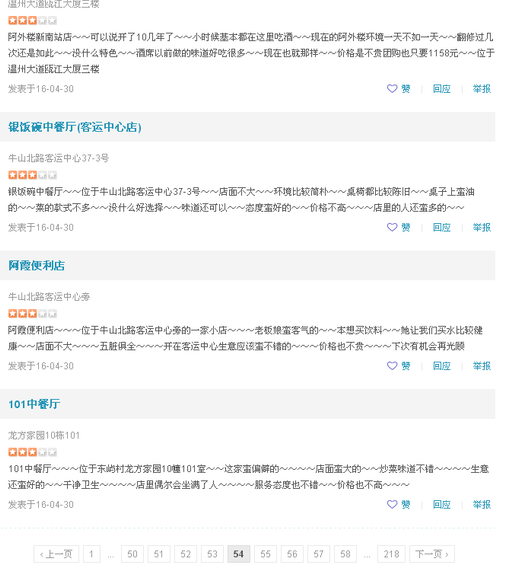
\includegraphics[height=8cm]{intro-4.jpg}}
	\caption[水军示例]{水军示例}
\end{figure}

水军检测方面的研究已经进行了数年\cite{Spirin:2012}。早期的水军形式非常基础,基本是脚本批量控制的机器水军,内容也非常简单,很容易人工辨别。如图~\ref{figure:bot-a}是典型的早期机器水军形式,其特点是用户名无意义或使用默认用户名,没有个性化信息(自定义头像等),使用大量不同的账号在短时间内发表几乎相同的内容等。这类早期机器水军由于特点鲜明,欺骗性低,很容易通过分析评论内容的方法分辨出来。早期的研究者们提出了许多基于文本的词法分析和语法分析方法,也有一些通过将评论和评论者特征应用于简单的机器学习算法来查找可疑账户的方法。Mukherjee等人 \parencite{Mukherjee:2013}分别利用词法分析方法和表现特征方法进行Yelp里的水军检测。在研究者们进行科研的同时,网络商业平台们也意识到了水军的危害性,并建立了各自的检测系统以过滤低质量评论和疑似水军评论。这些系统帮助维护了评论环境,但也促使水军技术的不断进步。机器水军逐渐落伍,人工水军凭借其隐蔽性优势逐渐成为水军主流。能够欺骗平台检测系统的水军技术层出不穷,甚至Yao等人 \parencite{Y.Yao:2017}研究出了用RNN(Recurrent Neural Networks)自动生成水军评论的方法,而且可以通过学习正常用户评论内容和控制生成速率的方法,躲避平台过滤系统的侦查。如图~\ref{figure:bot-b}就是大众点评上受雇佣的人工水军示例。单独来看每一条评论似乎与正常用户区别不大,但如果查看该用户每一条点评的时间就会发现他在一天只内写了数十条点评内容,这显然是不符合常理的。 在日益更新的水军技术面前,之前过时的水军检测技术急需更新。水军检测领域的着眼点也逐渐从文本分析转移到了模式提取和特征分析,时间、排名、话题度和活跃程度等特征也证明了它们检测水军的能力。这些新思路为水军检测领域提供了新的方向。Santosh等人 \parencite{Santosh:2016}在Yelp上分析了水军活动爆发出现的时间顺序和发生速率,并在此基础上提出了一个向量自回归(Vector AutoRegression)模型来预测水军活动的发生。他们认为水军的活动具有短时间内爆发的特征。这有这有才可以迅速达成水军们宣传雇主的目标。故这个爆发点可以用来预测水军的活动。Nilizadeh等人 \parencite{Nilizadeh:2017} 设计了一个利用用户喜好的话题来判别推特\footnote{www.twitter.com}中的可疑水军用户的模型。他们假设一个特定群体的用户所偏好的话题是固定的。若一个用户突然发布了一个他不偏好的话题的内容,那么他的身份就很可疑。

\section{SpamTracer水军检测模型}

本次毕业设计在前人工作的基础上,提出了自己的水军检测模型————\emph{SpamTracer}。该模型最大的特点是利用了地理位置特征。地理位置特征在水军检测方面具有很大的潜力。在O2O平台中,每家店铺都具有位置信息。用户评论过的所有店铺按照时间顺序形成序列,这些店铺的位置也会形成序列。无论是水军用户还是正常用户,只要参与过评论,都会形成这样的位置序列。但是,水军用户在进行水军活动的时候不会注意目标店铺的位置顺序,相邻店铺间的位置关系会比正常情况下更加复杂,即出现“绕远路”的现象。而普通用户评论种店铺的位置顺序是符合人类生活规律的。二者截然不同的行动理念产生的结果就是在地理位置相关特征的统计数据和分布情况上出现很大的差异。这种差异可以成为我们检测水军用户的切入点。而且,位置相关的特征难以伪造,可以有效防止水军绕开检测系统。通过在一个有标签的用户评论数据集上进行计算,我们发现水军用户和普通用户在地理特征上都表现出了双峰分布的特点。我们调整了SpamTracer模型使它能够完美契合这样的分布特点。

一些已经发表的工作也讨论过地理位置特征在水军检测方面的可能性。Zhang \parencite{Zhang:2014}等人在社交网络OSN(Online Social Networks)中利用地理位置特征检测水军账号。他们结合了账户特征(姓名、性别、评论数等)和位置信息,利用信息熵(Information Entropy)将二者结合进行判断。Gong等人 \parencite{Gong:2018}在基于位置的社交网络LBSN(Location-Based Social Networks)中收集了用户的签到(check-in)信息,然后利用LSTM(Long Short-Term Memory)神经网络分析这些签到信息,并在模型测试中展示出了极高的准确率。这些工作启发了我们,位置信息具有极大的潜力。我们的SpamTracer将使用全新的方法处理位置信息,并让这些特征在水军检测过程中起到关键作用。

除了水军检测以外,本次毕业设计还讨论了关于水军检测模型的应用。由于模型需要有大量的数据作为基础才能进行判断,而对于一般用户来说,并没有使用模型的条件。故我们可以利用SpamTracer分析水军用户们发动水军活动的时间规律和地点规律,这样就可以在一定程度上帮助普通用户鉴别水军。经过研究,我们发现网络商铺雇佣水军的行为确实存在一些时间规律和地点规律。例如:网络商铺倾向于在刚刚开业的时候雇佣水军帮助他们的店铺积累人气,并在平台的搜索系统中获得较高的排名。这样这些商铺就更有可能吸引到浏览的人的注意力,并获得更多的营业额。


\section{本次毕业设计的主要贡献}

本次毕业设计的主要贡献如下列出:

\begin{enumerate}
	\item[(1)] 我们使用地理位置特征在O2O商业平台中进行水军评论检测。我们收集了店铺的地理位置信息,按照时间顺序将属于同一个人点评过的店铺的位置信息整理在一起,形成地理位置特征序列。
	\item[(2)]  我们建立了一个特别的SpamTracer模型,用于描述水军用户和普通用户在地理位置特征上的分布差异。SpamTracer分析地理位置特征序列,然后对该用户所属身份(水军用户或普通用户)做出判断。
	\item[(3)]  我们提出了三个重要的水军行动的关于时间地点的命题。我们的实验结果证实了这些命题并给出了合理的解释。
\end{enumerate}

本文剩下的部分将按照如下说明开展:第二章介绍相关基础知识,包含机器学习相关、网络诈骗中的分类算法和隐马尔可夫模型简介;第三章介绍地理位置特征的具体提取步骤,并论述该特征的合理性;第四章介绍SpamTracer模型的建立过程,并论述该模型理论上的可行性;第五章介绍SpamTracer模型的应用,提出三条水军行动规律,并设计实验验证这些规律;第六章介绍模型的测试过程,包括数据集情况简介、实验环境描述、水军检测功能的测试结果及分析,以及水军行动规律分析实验的结果。最后,第七章得出结论,总结整个毕业设计。





%# -*- coding: utf-8-unix -*-
%%==================================================
%% chapter01.tex for SJTU Master Thesis
%%==================================================

%\bibliographystyle{sjtu2}%[此处用于每章都生产参考文献]
\chapter{前言}
\label{chap:preli}


\section{机器学习}

机器学习是一种赋予计算机学习能力,并让它完成直接编程无法完成的功能的方法。从实践角度讲,机器学习方法是利用已有的数据,得出某种模型,并利用此模型做预测的一种方法。机器学习可以视为模仿人类思考模式的过程。人类通过学习,积累知识经验,归纳生活规律。当人类遇到位置的问题或对未来进行推测时,就可以使用这些经验规律进行推测。机器学习中的“训练”和“预测”即对应人类的“归纳”和“推测”。

机器学习涉及的范围非常广阔。机器学习的基础包括概率论、数理统计、线性代数等。同时,机器学习可以作为工具,和其他领域的各种技术相结合,形成众多的交叉学科,包括数据挖掘、计算机视觉、语音识别技术、自然语言处理等。数据挖掘是利用机器学习处理海量数据的能力,从大量的数据中发现具有价值的东西;计算机视觉是机器学习与图像处理的结合,图像处理技术将图像处理为适合机器学习算法的输入,然后机器学习从图像中进行识别操作,例如手写识别等;语音识别技术是音频处理技术和机器学习的结合,例如苹果公司的Siri等;自然语言处理是让机器理解人类语言的学科,涉及词法分析、语法分析等编译相关的知识,是机器学习分类中备受瞩目的一个分支。

机器学习的算法种类五花八门。其中最为重要的算法主要分为以下几种类型:

\begin{enumerate}
	\item [(1)] \textbf{回归算法(Regression)}:代表为线性回归(Linear Regression)和逻辑回归(Logistic Regression)。线性回归指寻找一条直线可以最好地拟合数据,主要思想是最小二乘法。逻辑回归与线性回归相似,但线性回归的目标是预测一个数值,逻辑回归的目标是判断二分类。逻辑回归的主要思想是Sigmoid函数。
	\item [(2)] \textbf{神经网络(Neural Networks)}:神经网络本质是计算机模拟大脑的思考过程。神经网络对数据进行分解,由一层层的“神经元”处理数据,并把处理后的数据送给下一层神经元。每一个神经元都是一个逻辑回归模型,众多的神经元按层级结构组合起来,可以处理非常复杂的分类问题。神经网络的一个典型的应用就是手写数字识别问题(MNIST)。
	\item [(3)] \textbf{支持向量机(Support Vector Machine, SVM)}:SVM是对逻辑回归的优化,可以比逻辑回归更好地划分分类线。而且通过与核(Kernel)函数的结合,SVM可以在低维空间表达出高维空间的分类界限,在保留原本计算复杂性的条件下大大增强了分类的准确度。
	\item [(4)] \textbf{聚类算法}:前三类算法的基本条件是训练数据是有标签的数据,在训练后可以对同类型未标签的数据进行预测。而聚类算法是应用于无标签数据集上的算法,作用是计算数据群体中互相的间距,并根据间距的大小将数据划分为多个类别。K-Means算法就是典型的聚类算法。
\end{enumerate}

除了上述列出的算法以外,机器学习领域还有诸如用于决策的增强学习(Reinforcement Learning)、多隐藏层神经网络的深度学习(Deep Learning)等大型分支。机器学习是目前最火热的计算机科学领域之一。从AlphaGo到智能车自动驾驶,从谷歌识图到微软小冰,机器学习的实践应用也屡屡让世界惊叹。



\section{网络诈骗中的分类算法}

网络诈骗有多种类型,例如网页诈骗 \cite{Spirin:2012}、邮件诈骗 \cite{Castillo:2007}、远程通信诈骗 \cite{Yao:2017}和概念诈骗 \cite{Jindal:2008}。水军检测问题属于概念诈骗领域。面对这类问题,早期研究者们热衷于使用NLP和数据挖掘技术对各种概念进行分类和总结。后来他们试图优化文本分析方法,Shojaee等人 \parencite{Shojaee:2013}认为关注水军评论内容的词法特征和语法特点很关键。由于水军们试图模仿正常评论的内容来隐藏水军评论,所以他们的写作风格和用词风格一直在变化。因此,如果从文体形式出发来考虑的话,就可以辨别出水军评论的相似性,进一步找到那些虚假评论。他们提取出这些特征后使用经典的分类算法和进行检测。Chen等人 \parencite{Chen:2013}提出了基于语义分析的方法,用拆句子工具将评论内容拆分为一个个单词,并通过计算不同评论内容拆分后单词的相似数来衡量语义的相似程度。他们也尝试了使用非监督学习的方法进行检测,但效果并不是很好。

抛开NLP方法,在机器学习方法的帮助下,水军检测问题可以被视为二分类问题或排名问题。其中的关键部分便是特征的选取和模型的选取。可以在水军检测中应用的经典机器学习分类算法有很多:Ott等人 \parencite{Ott:2011}提出了SVM和单词条/双词条文本分析的结合,Chen等人 \parencite{CHEN:2009}提出了朴素贝叶斯NB(Naive Bayes)在文本分类问题中的应用。也有许多研究者在经典方法的基础上进行了改进,并提出了新的方法。Li等人 \parencite{Li:2014}提出了PU(Positive-Unlabeled)学习方法。他们认为在网络平台的过滤系统作用下,那些被过滤系统过滤掉的评论一定是虚假评论,然而被过滤系统判定为正常的评论中却还混有大量的虚假评论。故PU学习适用的数据集是那些只部分标记了一种类型数据,其他数据视为未标记数据的情况。他们还与大众点评公司合作,取得了珍贵的数据,在此基础上提出了新颖的模型。Chino等人 \parencite{Chino:2017}利用用户发布评论的时间间隔和评论内容量特征,训练了一个对数分布模型来拟合大众的特征分布情况,然后找到那些与主流分布隔离开来的点视作可疑用户。寻找与大众情况相异用户的思路非常新颖。Chen等人 \parencite{Chen:2017}提出了一个利用目标排名变动情况来寻找可疑用户的模型。如果目标短时间内在排行榜上发生了大幅震荡——排名迅速上升几天后又迅速下跌——那目标很可能雇佣了水军帮助他增长排名。不仅如此,他们还利用这一点进一步分析,成功捕捉到了水军团队。



\section{隐马尔可夫模型}

隐马尔可夫模型HMM(Hidden Markov Model)是一种经典的概率图模型。如图~\ref{fig:hmm},HMM可以用图来表示各个变量之间的关联。HMM有两个状态:观测态(图中$X_1 \cdots X_n$)和隐藏态(图中$Y_1 \cdots Y_n$)。隐藏态变量$Y_i$形成序列结构,然后每个隐藏态变量$Y_i$生成一个观测态变量$X_i$。在初始化时,HMM有一个初始状态概率(Initial State Probability)来决定由哪种隐藏态开始构建序列。之后每次出现一个新状态,隐藏态序列就增加一个变量,并且变量的值遵循一个特定的转移概率(Transition Probability)。隐藏态变量生成观测态变量的过程也遵循一个特定的输出概率(Emission Probability)。为了保证序列本身和各种概率的的合理性,HMM遵循两个重要的假设:
\begin{enumerate*}		
	\item[(1)] 每一个隐藏态变量的生成都只依赖于它之前的那一个隐藏态变量;
	\item[(2)] 每一个观测态变量的生成都只依赖于它对应的那个隐藏态变量。
\end{enumerate*}
这两个假设在大量的实践中被广泛认可。它们在不对结果产生重大影响的前提下大大简化了模型的计算复杂度。并且它们也保证了转移概率和输出概率的合理性。综上可知,一个特定的HMM序列可以由三个概率表示:初始状态概率、转移概率和输出概率。

\begin{figure}[htbp]
	\centering
	\begin{minipage}[htbp]{\textwidth}
		\centering
		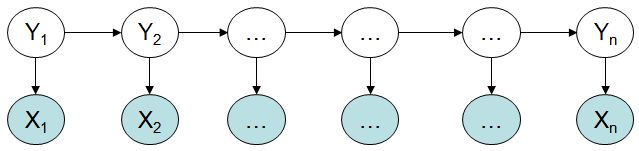
\includegraphics[width=10cm]{preli-1.jpg}
		\caption[HMM示例图]
		{HMM示例图\label{fig:hmm}}		
	\end{minipage}     
\end{figure}

用HMM解决的问题主要有三个类型:

\begin{enumerate}		
	\item[(1)] \textbf{参数估计}:给定一个观测序列,计算一组参数(三个概率)使该观测序列出现的可能性最大;
	\item[(2)] \textbf{由观测态序列确定隐藏态序列(解码问题)}:已知HMM模型,给定一个观测序列,求解最可能的隐藏序列;
	\item[(3)] \textbf{求解观测序列出现的概率}:已知HMM模型,给定一个观测序列,计算该序列出现的概率。
\end{enumerate}

参数估计问题可以视作HMM的训练问题。Rabiner在1989年提出了一种名为\emph{Baum-Welch}\cite{Rabiner:1989}的EM(Expectation-Modification)算法,利用极大似然估计方法来训练HMM参数,现在已经成为了该问题的普遍解决策略。由观测态序列确定隐藏态序列的问题在语音识别领域也称作解码问题,目标是在给定观测序列的情况下寻找概率最高的隐藏序列。Forney在1973年提出来了解决这种问题的\emph{Viterbi}\cite{Forney:1973}算法。计算观测序列概率的问题是计算特定HMM生成特定观测序列的概率。换句话说,这个问题可以用来计算观测序列和给定模型的关联程度。



%%# -*- coding: utf-8-unix -*-
%%==================================================
%% chapter01.tex for SJTU Master Thesis
%%==================================================

%\bibliographystyle{sjtu2}%[此处用于每章都生产参考文献]
\chapter{提取地理位置特征}
\label{chap:Featu}



\section{选择地理位置特征}

由于发布评论这个事件可以视为是以一个固定的概率稳定并独立发生的,故O2O平台的用户发布评论的过程可以视为一个随机过程。在这个随机过程下,评论相关的特征会遵循一些特殊的分布。例如著名的泊松过程下,时间间隔变量遵循泊松分布。在寻找帮助解决问题的特征时,研究目标特征遵循的分布特点十分有帮助。关于特征的选择,虽然已经有很多特征证明了它们在水军检测中的重要价值,例如时间、活跃量等,但是地理位置特征却被忽略了。地理位置特征是一项在水军检测任务中十分有潜力的特征,如果分别计算普通用户和水军用户的地理位置特征的相关统计数据和分布特点,加以分析并寻找它们之间的不同之处,那么地理位置特征就可以成为解决问题的切入点。经过我们的研究调查,我们发现了一个可用的地理位置特征——“半径”:

\begin{defn}
	\textbf{半径}:半径特征指每一个评论中店铺位置点和该用户的活动中心点的距离。其中用户的活动中心点是一个用户的评论列表中最活跃地区内各个店铺位置的地理中心。这个中心点可以被视为该用户的居所。
\end{defn}

图~\ref{fig:radius}是半径特征的示例,图中标有REVIEW LOCATION的点是一个用户写过评论的各个店铺的位置,标有CENTER的点是这些店铺位置的地理中心。我们认为这个点是该用户平时居住的地方,该用户的日常活动是以这个点为中心展开的。图中连接CENTER点和各个REVIEW LOCATION点的线代表了这些点的间隔距离,也就是每个店铺在该用户的评论中对应的半径特征的值。

\begin{figure}[htbp]
	\centering
	\begin{minipage}[htbp]{\textwidth}
		\centering
		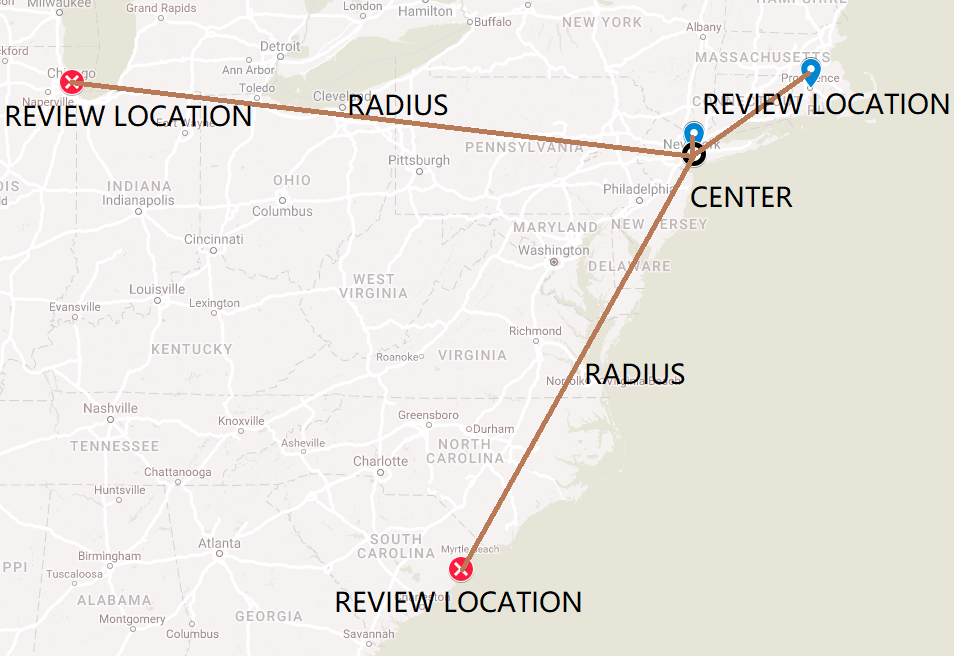
\includegraphics[width=10cm]{featu-1.png}
		\caption[地理位置特征“半径”示意图]
		{地理位置特征“半径”示意图(图源:谷歌地图)\label{fig:radius}}		
	\end{minipage}     
\end{figure}



\section{半径特征的合理性论述}

表~\ref{tbl:radius}和图~\ref{fig:hist}展示了半径特征的统计数据和频率分布直方图。计算数据来源于我们使用的数据集。统计数据中的平均值和标准差表现了半径特征在两类用户之间的差异。频率分布直方图更加具体地展示了水军用户(Spammer)和普通用户(Non-spammer)的差异,包括图像各位置的斜率、各顶点位置等。但是二者的图像也有相似的部分,那就是它们都呈现出了双峰分布的趋势。而这种双峰图像的形成过程可以看做是两个参数不同的高斯分布(Gaussian Distribution)在对数横坐标轴上的叠加。

\begin{table}[htbp]
	\caption{半径特征的统计数据}
	\label{tbl:radius}
	\centering
	\begin{tabular}{ccc}
		\toprule
		& 平均值 & 标准差  \\
		\midrule
		水军用户      & 310.0604  & 678.4959  \\
		普通用户  & 568.5133  &	999.4281 \\
		\bottomrule
	\end{tabular}
\end{table}

\begin{figure}[htbp]
	\centering
	\begin{minipage}[htbp]{\textwidth}
		\centering
		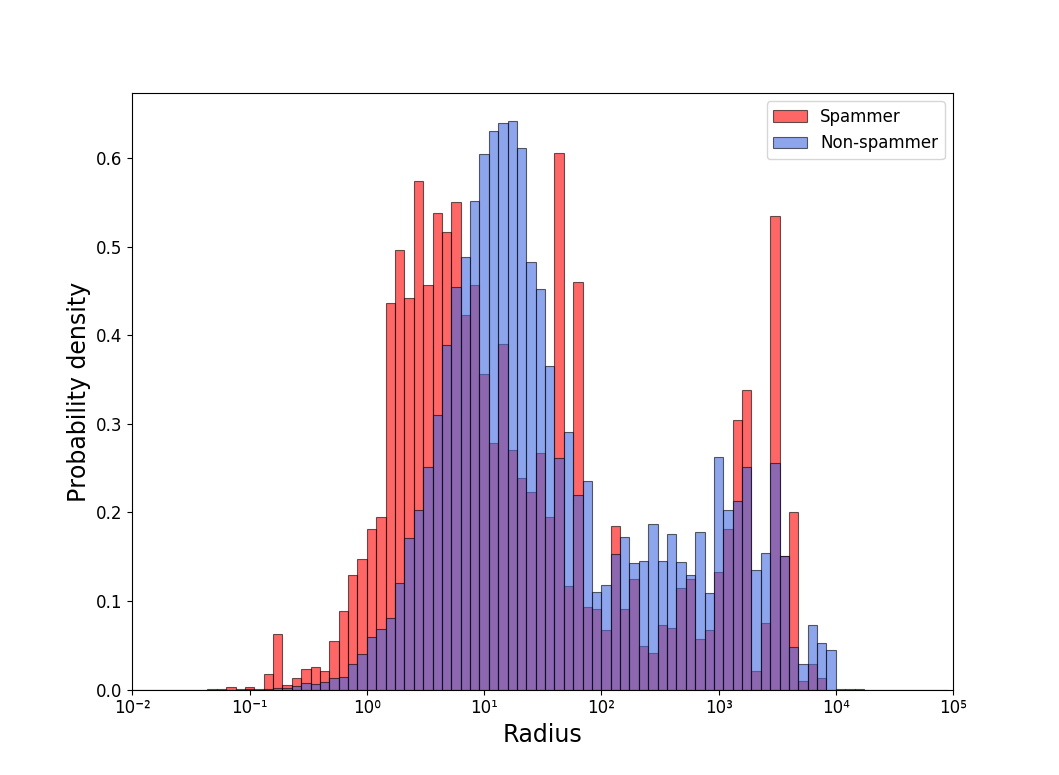
\includegraphics[width=10cm]{featu-2.png}
		\caption[半径特征的频率分布图]
		{半径特征的频率分布图\label{fig:hist}}		
	\end{minipage}     
\end{figure}

从水军用户和普通用户的行为上分析,这种双峰分布是合理的。一般来说,人类的活动范围可以分为两个模式:近距离活动和远距离活动。近距离活动就是人类在居所的附近活动,这类活动占比最高,活动范围不会很远,通常在一个城市的范围之内;远距离活动一般出现在一个人暂时离开居所的时候,例如旅游、出差等,这类活动的地理位置跨越范围较大,但持续时间不会太长。故普通用户图像中的双峰是近距离活动和远距离活动的合理体现。然而,水军用户并不符合近距离活动和远距离活动的模式,他们的行动模式是无规律的,水军用户的双峰图像只是其进行水军活动时不同半径的店铺数量占比的体现。此外,普通用户和水军用户在评论店铺的半径特征顺序上也是有差异的。普通用户评论过的店铺中,连续的店铺的半径特征值基本上是相近的。换句话说,普通用户在店铺的选择上具有空间连续性。这是因为人类的行动是具有空间连续性的,人们在一段时间内是在同一片区域生活的,所以人类日常消费的场所是接近的。即使短时间内出远门旅行,在旅行中的消费场所也是接近的。反观水军用户,其评论店铺的顺序是由雇主要求决定的而非人类正常活动,所以他们的半径特征不具有空间连续性。这两点关键差异将是SpamTracer模型进行水军检测的重要依据。

接下来对半径特征进行数学角度的建模。如上文所提到的,我们用两个参数不同的高斯分布的叠加来描述半径特征的频率分布。假设$x_i, i = 1,...,T$是一个用户的评论列表中按时间排序出现的店铺位置,根据公式~\eqref{equation:1},我们计算其地理中心$C$,然后计算每一个评论的店铺所对应的半径特征值$\gamma_{x_i}$。半径特征值$\gamma_{x_i}$遵循高斯分布。


\begin{equation}
\label{equation:1}
\begin{aligned}
& C = (\frac{\sum_{t \in T}{x_t.latitude}}{|T|}, \frac{\sum_{t \in T}{x_t.longitude}}{|T|})\\
& \gamma_{x_i} = Distance(x_i, C)\\
& f(x;\mu, \sigma) = \frac{1}{\sqrt{2\pi}\sigma}\exp{(-\frac{(x-\mu)^2}{2\sigma^2})} \qquad
\gamma_{x}\sim N(\mu, \sigma^2) \\
\end{aligned}
\end{equation}
%# -*- coding: utf-8-unix -*-
%%==================================================
%% chapter01.tex for SJTU Master Thesis
%%==================================================

%\bibliographystyle{sjtu2}%[此处用于每章都生产参考文献]
\chapter{建立SpamTracer检测模型}
\label{chap:model}


\section{模型整体结构}

本节我们要介绍SpamTracer水军检测模型的设计结构和设计理念。如图~\ref{fig:structure}所示为SpamTracer模型的水军检测流程图。整个检测流程分为以下四个步骤:

\begin{figure}[htbp]
	\centering
	\begin{minipage}[htbp]{0.6\textwidth}
		\centering
		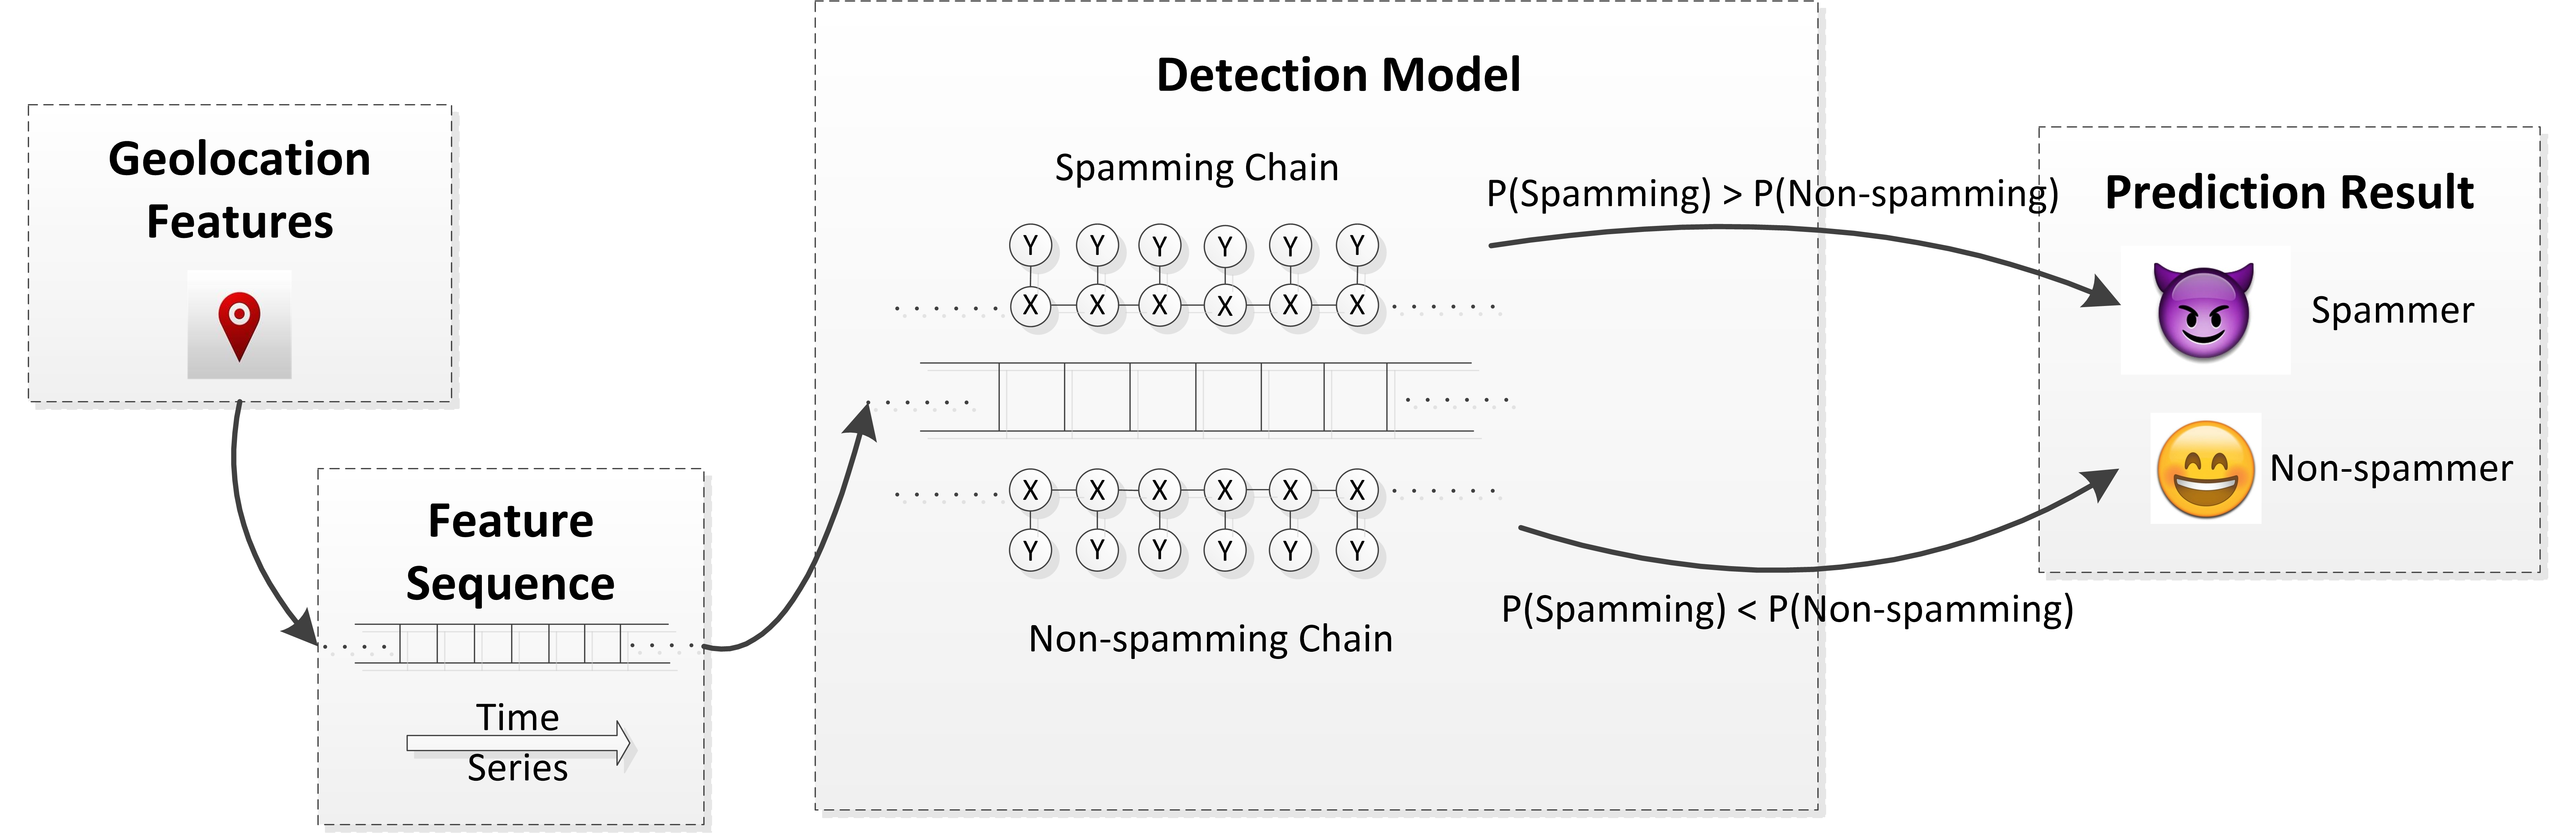
\includegraphics[width=10cm]{model-1.jpg}
		\caption[水军检测流程图]
		{水军检测流程图\label{fig:structure}}		
	\end{minipage}     
\end{figure}

\begin{enumerate}
	\item[(1)] 从数据集中提取地理位置信息数据;
	\item[(2)] 计算每个用户的评论中出现的店铺的半径特征,将计算结果按照时间顺序排序,形成特征序列;
	\item[(3)] 将待检测用户的特征序列输入模型;
	\item[(4)] 模型输出该用户是否为水军用户的判断结果。
\end{enumerate}

SpamTracer做出判断是依据概率。在输入特征序列后,SpamTracer会根据训练出的参数,分别计算该序列属于水军用户的概率和普通用户的概率,然后选择概率较大的一方作为判断结果。下文将会叙述SpamTracer的设计理念,以及模型具体如何进行计算。



\section{建立模型}

接下来我们将叙述如何对地理位置特征进行建模。我们之所以使用半径特征序列而非单独的半径特征,是因为序列可以反映上一章所提到的空间连续性,这是分辨普通用户和水军用户的重要依据之一。而且,比起单独的特征,序列形式的特征的有序性可以最大化用户之间的区分度。为了充分利用地理位置特征序列,我们在HMM的基础上进行了改造,设计了处理半径特征序列的监督模型——SpamTracer。

\begin{figure}[htbp]
	\centering
	\begin{minipage}[htbp]{0.6\textwidth}
		\centering
		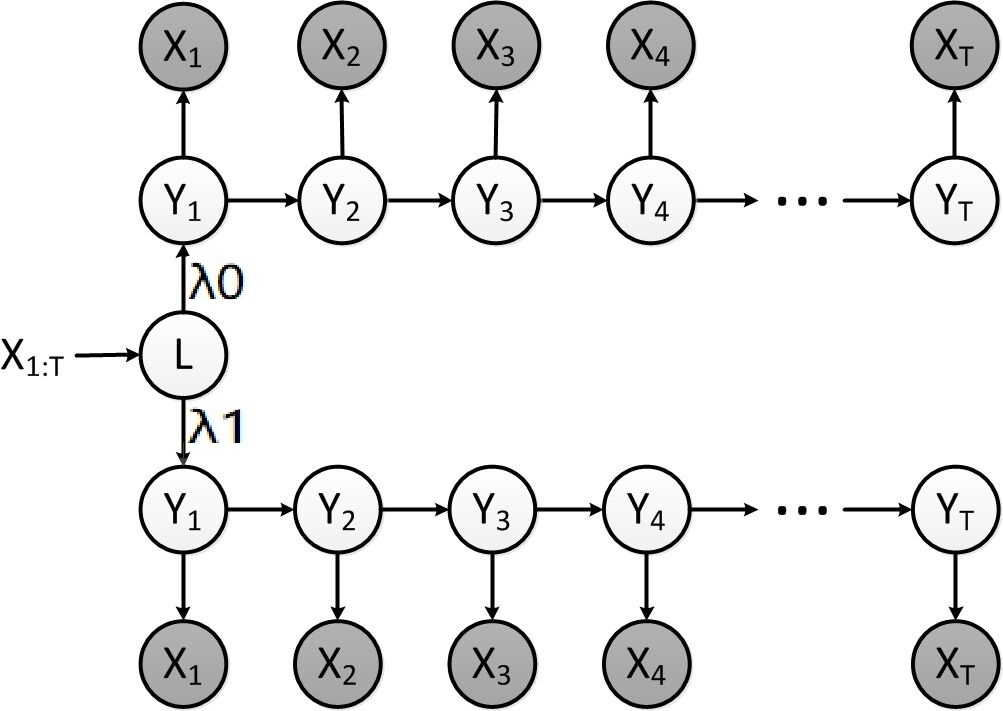
\includegraphics[width=10cm]{model-2.jpg}
		\caption[SpamTracer的双链结构]
		{SpamTracer的双链结构\label{fig:lhmm}}		
	\end{minipage}     
\end{figure}


如图~\ref{fig:lhmm}所示,SpamTracer包含两个HMM子链,以及一个连接两个子链的标签变量。标签变量标记为$L\in\{0,1\}$,其中$0$代表普通用户类,$1$代表水军用户类。两个子链标记为$\lambda_{0}$ = \{$\mathbf{A}_0$, $\mathbf{B}_0$, $\mathbf{\pi_0}$\} 和 $\lambda_{1}$ = \{$\mathbf{A}_1$, $\mathbf{B}_1$, $\mathbf{\pi_1}$\},分别代表普通用户和水军用户,并由相对应类型的数据进行训练。当输入一个新的特征序列时,两个子链会计算各自生成这个序列的概率。这个概率可以视为用来衡量该特征序列与对应子链类别相合程度的分数。分数计算完毕后,模型将比较两个分数的大小,并取拥有较大分数的类别作为判断结果。


\section{模型的合理性分析}


接下来我们将从数学角度论证SpamTracer检测过程的合理性。假设有一个位置标签$L$的特征序列$X_{1:T}$输入模型,我们的目的是计算该序列对应标签$L\in\{0,1\}$在不同取值时的产生概率。如公式~\eqref{equation:11}所示,根据贝叶斯公式(Bayes Theorem),计算给定特征序列列$X_{1:T}$条件下标签类型$L = l$的概率$P(L=l|X_{1:T})$可以转化为计算对应子链$\lambda_l$生成给定特征序列列$X_{1:T}$的概率$P(X_{1:T} | \lambda_l)$。此外,公式中的分母部分$P(X_{1:T})$是一个与标签$L$无关的值,故这是一个常量,在比较大小的过程中我们可以忽略它;$P(L = l)$的概率我们可以简单地通过统计数据集中标签为$l$的样本的个数获得。于是问题的关键就在于如何计算不同子链下产生给定特征序列$X_{1:T}$的概率$P(X_{1:T} | \lambda_l)$。

\begin{equation}
\label{equation:11}
\begin{aligned}
\widehat{L} & = \max_{l}{P(L = l| X_{1:T})} \\
& = \max_{l}{\frac{P(X_{1:T} | \lambda_l) \cdot P(L = l)}{P(X_{1:T})}}, l\in \{0,1\}
\end{aligned}
\end{equation}

假设$x_i, i = 1,...,T$是一个用户的评论列表中按时间排序出现的店铺位置,$\gamma_{x_i}$代表每一个评论的店铺所对应的半径特征值。在SpamTracer的子链中,$\gamma_{x_i}$充当了连续的观测态变量$X_i$,即$X_i = \gamma_{x_i}$。$\gamma_{x_i}$遵从两个不同的高斯分布,具体遵从哪一个则是由对应的隐藏态决定的。隐藏态变量值$Y_i$代表$x_i$的模式。$Y_i$有两个可能的取值$\{0,1\}$,分别代表上一章提到的近距离活动模式和远距离活动模式。

子链是由三个参数决定的:初始化概率$\mathbf{\pi}$、转移概率$\mathbf{A}$和输出概率$\mathbf{B}$。初始化概率$\mathbf{\pi} = \{\pi_j\} = \{P(Y_i = j)\}, j \in \{0,1\}$。由于隐藏态的转移概率仅仅依赖于上一个隐藏态,故转移概率如公式~\eqref{equation:3}所示。

\begin{equation}
\label{equation:3}
\mathbf{A} = \{a_{jk}\} = 
\begin{bmatrix}
a_{0,0}	&	a_{0,1}	\\
a_{1,0}	&	a_{1,1}	\\
\end{bmatrix}
\end{equation}

观测态变量$X_i$可以直接从数据集中获得,但是$X_i$本质上是由两种不同的高斯分布中的一种生成的,其中高斯分布的种类由对应的隐藏态变量决定$Y_i \in \{0,1\}$。公式~\eqref{equation:5}展示了观测态变量$X_i$是如何服从分布的。

\begin{equation}
\label{equation:5}
X_i = \gamma_{x_i} \sim 
\begin{cases}
N(\mu_0, \sigma_0^2)     &     Y_i = 0	\\
N(\mu_1, \sigma_1^2)     &     Y_i = 1	\\
\end{cases} 	
\end{equation}

与公式~\eqref{equation:1}结合起来看,输出概率$\mathbf{B}$可以用公式~\eqref{equation:6}计算而得。


\begin{equation}
\label{equation:6}
b_j(X_i) = b_j(\gamma_{x_i}) = P(\gamma_{x_i} | Y_i = j) = f(\gamma_{x_i};\mu_j, \sigma_j) \quad j \in \{0,1\}
\end{equation}

综上,我们论述了每个子链$\lambda$及其各自参数$\{\mathbf{A}, \mathbf{B}, \mathbf{\pi}\}$的计算过程,以及如何适配半径特征$\gamma_{x_i}$的分布情况。接下来我们开始计算生成特征序列的生成概率。如果用$X_{1:T}$代表从$x_1$到$x_T$的观测态序列,$Y_{1:T}$代表从$x_1$到$x_T$的隐藏态序列,则公式~\eqref{equation:7}可以计算$X_{1:T}$和$Y_{1:T}$的联合概率。概率$P(X_{1:T}, Y_{1:T})$的含义是$X_{1:T}$和$Y_{1:T}$都按照顺序出现在第$1$到第$T$个位置上的概率。这个计算过程的时间复杂度是$O(T)$。


\begin{equation}
\label{equation:7}
\begin{aligned}
& P(X_{1:T}, Y_{1:T})\\
= & P(Y_1, X_1, Y_2, X_2,...,Y_T, X_T)\\
= & P(Y_1)\prod_{i=1}^{T}{P(X_i|Y_i)}\prod_{i=2}^{T}{P(Y_i|Y_{i-1})}\\
= & \pi_{Y_1}\prod_{i=1}^{T}{b_i(X_i)}\prod_{i=2}^{T}{a_{Y_i Y_{i-1}}}
\end{aligned}
\end{equation}


然而,在实际情况下,对于任意一个给定的观测态序列$X_{1:T}$,我们是不知道它对应的隐藏态序列$Y_{1:T}$的。所以SpamTracer在计算中必须考虑隐藏态序列列$Y_{1:T}$所有的排列组合,共$2^T$中不同的可能性。在这种情况下,计算联合概率的公式如公式~\eqref{equation:8}所示:

\begin{equation}
\label{equation:8}
\begin{aligned}
& P(X_{1:T})\\
= & \sum_{Y_{1:T}} P(X_{1:T}, Y_{1:T})\\
= & \sum_{Y_{1:T}} P(Y_1)\prod_{i=1}^{T}{P(X_i|Y_i)}\prod_{i=2}^{T}{P(Y_i|Y_{i-1})}
\end{aligned}
\end{equation}

如果直接按照上述公式进行计算,时间复杂度将会达到$O(T\cdot2^T)$。这是几乎接近不可计算等级的复杂度。造成如此高计算复杂度的原因主要是该公式对许多中间量进行了冗余的计算。如果能够在计算过程中保存部分中间量,计算将被大大简化。基于这个思路,存在一个典型的算法Forward-backward算法 \cite{Rabiner:1989}。这个算法可以将公式~\eqref{equation:8}的时间复杂度优化为线性复杂度,大大节省了计算成本。

综上所述,计算不同子链下产生给定特征序列$X_{1:T}$的概率$P(X_{1:T} | \lambda_l)$是完全可行的。我们在理论上证明了SpamTracer是完全可以作为一个监督模型胜任分类工作的。SpamTracer给出的打分可以作为水军检测的依据。



\include{tex/Appli}
%# -*- coding: utf-8-unix -*-
%%==================================================
%% chapter01.tex for SJTU Master Thesis
%%==================================================

%\bibliographystyle{sjtu2}%[此处用于每章都生产参考文献]
\chapter{模型性能测试}
\label{chap:exper}



\section{数据集描述}

正确选择数据集是实验成功的关键,与模型要求相合的数据集可以助实验事半功倍。首先我们考虑了自己编写爬虫程序爬取数据的可能性,但是这种做法没办法取得标签信息,如果人工进行标签处理是一件十分枯燥且主观成分浓厚的事情,这对于实验是没有好处的。经过讨论,我们还是选择了使用别人收集好的数据集。前人的工作中有很多已经整理好的数据集,而且各有特色。Jindal等人 \parencite{Jindal:2008}发布了一个亚马逊的评论数据集,但是亚马逊平台与我们模型的目标不合;Li等人 \parencite{Li:2014}与大众点评公司合作,发布了一个大众点评的数据集,但是这个数据集没有包含店铺的位置信息;Rayana等人 \parencite{Rayana:2015}发布了一个自己搜集的Yelp数据集,包含店铺的评论信息和Yelp过滤系统给这些评论打的标签,但是这个数据集中的评论是按照店铺归类的。还有很多其他的数据集,都与我们实验的设想有很大差异。

最后,我们找到了Santosh等人 \parencite{Santosh:2016}使用过的Yelp数据集。这是一个部分标签的数据集,包含店铺的地址信息,而且评论信息也按照评论账户做了归类,非常适合我们的模型。数据集的标签部分中,每一条评论都被Yelp的过滤系统分类为了“虚假评论”和“普通评论”。数据集的相关数据如表~\ref{tbl:dataset}所示,数据集中一共含有760212条评论和16941个用户,其中带标签的评论有107624条,所有评论都被打过标签的用户有3142个。在107624条带标签评论中,20267条是虚假评论。这个数据集还有一个特色,那就是每一个被打过标签的用户的过滤比(即该用户所有评论中虚假评论的占比)都在0-20\%或90-100\%区间内。由于数据集本身并没有对用户进行标签处理,所以我们定义过滤比大于90\%的用户为水军用户,过滤比小于20\%的用户为普通用户。在这个分类标准下,3124个所有评论都被打过标签的用户中有1299个水军用户。此外,为了减少测试误差,一些发表评论数过低的用户将被过滤掉,不参与实际的计算。将评论数阈值设置为5的话,参与计算的用户数量将剩下11917个,所有评论都被打过标签的用户只剩下1796个。

\begin{table}[htbp]
	\caption[数据集相关数据]{数据集相关数据}
	\label{tbl:dataset}
	\centering
	\begin{tabular}{ccc}
		\toprule
		& 带标签的个数 & 总数  \\
		\midrule
		评论数  & 107624  & 760212  \\
		用户数  & 3142  &	16941 \\
		水军评论数 & 20267 & N/A \\
		水军用户数 & 1299 & N/A \\
		过滤后用户数 & 1796 & 11917 \\
		\bottomrule
	\end{tabular}
\end{table}

\section{实验描述}

本节我们将介绍实验的设置。实验环境的配置如表~\ref{tab:environment}所示。

\begin{table}[htbp]
	\caption[实验环境]{实验环境}
	\label{tab:environment}
	\centering
	\begin{tabular}{| c | c |}
		\hline
		\centering
		操作系统 &  Mac OS 10.12.6\\
		\hline
		\centering
		内存 & 8GB 1600MZ DDR3\\
		\hline
		\centering
		显卡 & Intel HD Graphics 6000 1536MB\\
		\hline
		\centering
		CPU & 1.6GHz Intel Core i5\\
		\hline
		\centering
		数据库软件 & Mysql v14.14\\
		\hline
		\centering
		模型编写 & Python 2.7 + pomegranate +
		scikit-learn\\
		\hline
	\end{tabular}
\end{table}

模型使用的地理位置特征是通过经纬度计算出来的,店铺的经纬度是使用一个名为\emph{geocoder}的python库,利用\emph{Arcgis}地图提供的地理位置编码功能从地址转换而来的。SpamTracer的模型参数是利用训练集训练得到的,测试是基于测试数据集的。训练集和测试数据集是数据集中包含标签部分内的不相交的两个集合。一个严重的问题是,数据集内的普通数据量和水军数据量是不平衡的,比例约为3:1,而实际上O2O平台的水军用户相比于普通用户也是占少数的那部分。在这样不平衡的数据集下,分类器需要能够抵挡数据的不平衡带来的影响。许多传统的分类算法在不平衡数据集中不能正常发挥,而SpamTracer可以经受大量误导数据的影响,准确地检测出小部分水军。

我们设计了对照组来测试SpamTracer的各项指标,这些对照组都是经典的分类方法。公平起见,我们选择的对照组都是监督型(Supervised)的算法,和SpamTracer的类型一致。对照组包含四个分类器:朴素贝叶斯NB、聚类算法AdaBoost、支持向量机SVM和多层感知机MLP(Multi-layer Perceptron)。对照组的模型使用用户的账户相关特征作为检测依据,包括评论数量、账号的朋友数量、账号的粉丝数量、被选为优质评论的数量等。所有模型在测试中都使用10层交叉验证(Cross Validation)以保证测试结果的可靠性。



\section{模型测试结果}




\section{水军行动规律验证}
%# -*- coding: utf-8-unix -*-
%%==================================================
%% chapter01.tex for SJTU Master Thesis
%%==================================================

%\bibliographystyle{sjtu2}%[此处用于每章都生产参考文献]
\chapter{结论}
\label{chap:concl}


在这篇论文中,我们进行了利用地理位置特征检测O2O商业平台中水军的研究。我们分七章介绍了我们的工作。在第一章绪论中,我们简单介绍了水军检测领域的问题背景,介绍了当前互联网产业的飞速发展,以及水军对于电商平台的巨大为黑,阐述了我们的研究的重要性。之后我们介绍了水军检测领域的研究现状,介绍了众多前人的工作,并在前人工作的基础上提出了自己的想法——我们利用地理位置特征作为切入点,建立模型进行水军检测工作。在第二章前言部分,我们简单介绍了本文中用到的知识基础——机器学习相关理论、水军检测领域的分类模型以及隐马尔可夫模型。机器学习方法是本篇论文中的主要思路,应用在水军检测领域的相关模型给我们提供思路,而隐马尔可夫模型是我们模型的基础。在掌握了基础知识之后,我们在第三章详细地介绍了地理位置特征的提取。地理位置特征是我们的检测模型中至关重要的一环,选择怎么样的地理位置特征直接关系检测效果。我们提出了一个类似“半径”的地理位置特征,并用统计数据和分布数据支持了“半径”特征的可靠性。在第四章中,我们提出了一个可以利用“半径”特征的检测模型——SpamTracer。SpamTracer基于隐马尔可夫模型,我们将隐马尔可夫模型改造为了监型督分类模型。SpamTracer输入一个用户所有评论的按时间顺序排序的“半径”特征序列,根据训练数据分别计算该特征序列属于普通用户或水军用户的概率,最后比较概率大小输出判断结果。我们在数学上推导了概率的计算过程,证明了模型的可实践性。在第五章中,我们利用提出的SpamTracer模型,进行了水军行动规律的探索。我们使用SpamTracer扩展了数据集,给所有未标签的评论都打了标签,并提出算法使用这些数据分析水军在时间上和地理位置上的行动规律。在第六章中,我们首先介绍了选择数据集的过程,以及最后采用的数据集的特点。我们使用的数据集是一个部分标签的Yelp数据集,包含店铺信息、评论信息和用户信息。我们从这个数据集里提取出我们需要的特征序列,将带标签的数据输入SpamTracer模型进行训练并测试准确率。为了体现出SpamTracer的优势,我们选择了四个经典分类算法——朴素贝叶斯分类器NB、支持向量机SVM、AdaBoost分类器和多层感知机MLP。我们以广泛使用的四项测试指标,精确度Precision、召回率Recall、准确率Accuracy和F1值,使用10层交叉验证方法对SpamTracer和对照组模型进行了测试。测试结果显示在不平衡数据集中,SpamTracer的优秀的稳定性和准确率获得了最好的表现。同时,我们也发现了SpamTracer仍然有进步空间,我们分析了SpamTracer模型的不足之处,提出了可能的限制因素。此外,我们还公布了我们关于水军行动规律分析的实验结果。我们发现水军倾向于在一年中的夏季和一周中的周末进行水军活动,在店铺的开业初期进行水军活动。我们还发现了不同店铺间共有水军的数量与店铺的间隔距离成反比例关系,这说明小部分水军会在一个小商圈内与多家店铺进行合作。


%%# -*- coding: utf-8-unix -*-
%%==================================================
%% chapter02.tex for SJTU Master Thesis
%% based on CASthesis
%% modified by wei.jianwen@gmail.com
%% Encoding: UTF-8
%%==================================================

\chapter{{\LaTeX} 排版例子}
\label{chap:example}

\section{列表环境}
\label{sec:list}

\subsection{无序列表}
\label{sec:unorderlist}

以下是一个无序列表的例子,列表的每个条目单独分段。

\begin{itemize}
  \item 这是一个无序列表。
  \item 这是一个无序列表。
  \item 这是一个无序列表。
\end{itemize}

使用\verb+itemize*+环境可以创建行内无序列表。
\begin{itemize*}
  \item 这是一个无序列表。
  \item 这是一个无序列表。
  \item 这是一个无序列表。
\end{itemize*}
行内无序列表条目不单独分段,所有内容直接插入在原文的段落中。

\subsection{有序列表}
\label{sec:orderlist}

使用环境\verb+enumerate+和\verb+enumerate*+创建有序列表,
使用方法无序列表类似。

\begin{enumerate}
  \item 这是一个有序列表。
  \item 这是一个有序列表。
  \item 这是一个有序列表。
\end{enumerate}

使用\verb+enumerate*+环境可以创建行内有序列表。
\begin{enumerate*}
  \item 这是一个默认有序列表。
  \item 这是一个默认有序列表。
  \item 这是一个默认有序列表。
\end{enumerate*}
行内有序列表条目不单独分段,所有内容直接插入在原文的段落中。

\subsection{描述型列表}

使用环境\verb+description+可创建带有主题词的列表,条目语法是\verb+\item[主题] 内容+。
\begin{description}
    \item[主题一] 详细内容
    \item[主题二] 详细内容
    \item[主题三] 详细内容 \ldots
\end{description}

\subsection{自定义列表样式}

可以使用\verb+label+参数控制列表的样式,
详细可以参考WikiBooks\footnote{\url{https://en.wikibooks.org/wiki/LaTeX/List_Structures\#Customizing_lists}}。
比如一个自定义样式的行内有序列表
\begin{enumerate*}[label=\itshape\alph*)\upshape]
  \item 这是一个自定义样式有序列表。
  \item 这是一个自定义样式有序列表。
  \item 这是一个自定义样式有序列表。
\end{enumerate*}

\section{数学排版}
\label{sec:matheq}

\subsection{公式排版}
\label{sec:eqformat}

这里有举一个长公式排版的例子,来自\href{http://www.tex.ac.uk/tex-archive/info/math/voss/mathmode/Mathmode.pdf}{《Math mode》}:

\begin {multline}
  \frac {1}{2}\Delta (f_{ij}f^{ij})=
  2\left (\sum _{i<j}\chi _{ij}(\sigma _{i}-
    \sigma _{j}) ^{2}+ f^{ij}\nabla _{j}\nabla _{i}(\Delta f)+\right .\\
  \left .+\nabla _{k}f_{ij}\nabla ^{k}f^{ij}+
    f^{ij}f^{k}\left [2\nabla _{i}R_{jk}-
      \nabla _{k}R_{ij}\right ]\vphantom {\sum _{i<j}}\right )
\end{multline}

\subsection{SI单位}

使用\verb+siunitx+宏包可以方便地输入SI单位制单位,例如\verb+\SI{5}{\um}+可以得到\SI{5}{\um}。

\subsubsection{一个四级标题}
\label{sec:depth4}

这是全文唯一的一个四级标题。在这部分中将演示了mathtools宏包中可伸长符号(箭头、等号的例子)的例子。

\begin{displaymath}
    A \xleftarrow[n=0]{} B \xrightarrow[LongLongLongLong]{n>0} C 
\end{displaymath}

\begin{eqnarray}
  f(x) & \xleftrightarrow[]{A=B}  & B \\
  & \xleftharpoondown[below]{above} & B \nonumber \\
  & \xLeftrightarrow[below]{above} & B
\end{eqnarray}

又如:

\begin{align}
  \label{eq:none}
  & I(X_3;X_4)-I(X_3;X_4\mid{}X_1)-I(X_3;X_4\mid{}X_2) \nonumber \\
  = & [I(X_3;X_4)-I(X_3;X_4\mid{}X_1)]-I(X_3;X_4\mid{}\tilde{X}_2) \\
  = & I(X_1;X_3;X_4)-I(X_3;X_4\mid{}\tilde{X}_2)
\end{align}

\subsection{定理环境}

模板中定义了丰富的定理环境
algo(算法),thm(定理),lem(引理),prop(命题),cor(推论),defn(定义),conj(猜想),exmp(例),rem(注),case(情形),
bthm(断言定理),blem(断言引理),bprop(断言命题),bcor(断言推论)。
amsmath还提供了一个proof(证明)的环境。
这里举一个“定理”和“证明”的例子。
\begin{thm}[留数定理]
\label{thm:res}
  假设$U$是复平面上的一个单连通开子集,$a_1,\ldots,a_n$是复平面上有限个点,$f$是定义在$U\backslash \{a_1,\ldots,a_n\}$上的全纯函数,
  如果$\gamma$是一条把$a_1,\ldots,a_n$包围起来的可求长曲线,但不经过任何一个$a_k$,并且其起点与终点重合,那么:

  \begin{equation}
    \label{eq:res}
    \ointop_{\gamma}f(z)\,\mathrm{d}z = 2\uppi\mathbf{i}\sum^n_{k=1}\mathrm{I}(\gamma,a_k)\mathrm{Res}(f,a_k)
  \end{equation}

  如果$\gamma$是若尔当曲线,那么$\mathrm{I}(\gamma, a_k)=1$,因此:

  \begin{equation}
    \label{eq:resthm}
    \ointop_{\gamma}f(z)\,\mathrm{d}z = 2\uppi\mathbf{i}\sum^n_{k=1}\mathrm{Res}(f,a_k)
  \end{equation}

      % \oint_\gamma f(z)\, dz = 2\pi i \sum_{k=1}^n \mathrm{Res}(f, a_k ). 

  在这里,$\mathrm{Res}(f, a_k)$表示$f$在点$a_k$的留数,$\mathrm{I}(\gamma,a_k)$表示$\gamma$关于点$a_k$的卷绕数。
  卷绕数是一个整数,它描述了曲线$\gamma$绕过点$a_k$的次数。如果$\gamma$依逆时针方向绕着$a_k$移动,卷绕数就是一个正数,
  如果$\gamma$根本不绕过$a_k$,卷绕数就是零。

  定理\ref{thm:res}的证明。
  
  \begin{proof}
    首先,由……

    其次,……

    所以……
  \end{proof}
\end{thm}

上面的公式例子中,有一些细节希望大家注意。微分号d应该使用“直立体”也就是用mathrm包围起来。
并且,微分号和被积函数之间应该有一段小间隔,可以插入\verb+\,+得到。
斜体的$d$通常只作为一般变量。
i,j作为虚数单位时,也应该使用“直立体”为了明显,还加上了粗体,例如\verb+\mathbf{i}+。斜体$i,j$通常用作表示“序号”。
其他字母在表示常量时,也推荐使用“直立体”譬如,圆周率$\uppi$(需要upgreek宏包),自然对数的底$\mathrm{e}$。
不过,我个人觉得斜体的$e$和$\pi$很潇洒,在不至于引起混淆的情况下,我也用这两个字母的斜体表示对应的常量。


\section{向文档中插入图像}
\label{sec:insertimage}

\subsection{支持的图片格式}
\label{sec:imageformat}

\XeTeX 可以很方便地插入PDF、PNG、JPG格式的图片。

插入PNG/JPG的例子如\ref{fig:SRR}所示。
这两个水平并列放置的图共享一个“图标题”(table caption),没有各自的小标题。

\begin{figure}[!htp]
  \centering
  
\includegraphics[width=4cm]{example/sjtulogo.png}
  \hspace{1cm}
  
\includegraphics[width=4cm]{example/sjtulogo.jpg}
  \bicaption[这里将出现在插图索引中]
    {中文题图}
    {English caption}
  \label{fig:SRR}
\end{figure}

这里还有插入EPS图像和PDF图像的例子,如图\ref{fig:epspdf:a}和图\ref{fig:epspdf:b}。这里将EPS和PDF图片作为子图插入,每个子图有自己的小标题。子图标题使用subcaption宏包添加。

\begin{figure}[!htp]
  \centering
  \subcaptionbox{EPS 图像\label{fig:epspdf:a}}[3cm] %标题的长度,超过则会换行,如下一个小图。
    {
\includegraphics[height=2.5cm]{example/sjtulogo.eps}}
  \hspace{4em}
  \subcaptionbox{PDF 图像,注意这个图略矮些。如果标题很长的话,它会自动换行\label{fig:epspdf:b}}
    {
\includegraphics[height=2cm]{sjtulogo.pdf}}
  \bicaption{插入eps和pdf的例子(使用 subcaptionbox 方式)}{An EPS and PDF demo with subcaptionbox}
  \label{fig:pdfeps-subcaptionbox}
\end{figure}

\begin{figure}[!htp]
  \centering
  \begin{subfigure}{2.5cm}
    \centering
    
\includegraphics[height=2.5cm]{example/sjtulogo.eps}
    \caption{EPS 图像}
  \end{subfigure}
  \hspace{4em}
  \begin{subfigure}{0.4\textwidth}
    \centering
    
\includegraphics[height=2cm]{sjtulogo.pdf}
    \caption{PDF 图像,注意这个图略矮些。subfigure中同一行的子图在顶端对齐。}
  \end{subfigure}
  \bicaption{插入eps和pdf的例子(使用 subfigure 方式)}{An EPS and PDF demo with subfigure}
  \label{fig:pdfeps-subfigure}
\end{figure}

更多关于 \LaTeX 插图的例子可以参考\href{http://www.cs.duke.edu/junhu/Graphics3.pdf}{《\LaTeX 插图指南》}。

\subsection{长标题的换行}
\label{sec:longcaption}

图\ref{fig:longcaptionbad}和图\ref{fig:longcaptiongood}都有比较长图标题,通过对比发现,图\ref{fig:longcaptiongood}的换行效果更好一些。
其中使用了minipage环境来限制整个浮动体的宽度。

\begin{figure}[!htp]
  \centering
  
\includegraphics[width=4cm]{sjtubadge.pdf}
  \bicaption[这里将出现在插图索引]
    {上海交通大学是我国历史最悠久的高等学府之一,是教育部直属、教育部与上海市共建的全国重点大学.}
    {Where there is a will, there is a way.}
 \label{fig:longcaptionbad}
\end{figure}

\begin{figure}[!htbp]
  \centering
  \begin{minipage}[b]{0.6\textwidth}
    \centering
    
\includegraphics[width=4cm]{sjtubadge.pdf}
    \caption[出现在插图索引中]
      {上海交通大学是我国历史最悠久的高等学府之一,是教育部直属、教育部与上海市共建的全国重点大学.}
      {Where there is a will, there is a way.}
    \label{fig:longcaptiongood}
  \end{minipage}     
\end{figure}

\subsection{绘制流程图}

图\ref{fig:flow_chart}是一张流程图示意。使用tikz环境,搭配四种预定义节点(\verb+startstop+、\verb+process+、\verb+decision+和\verb+io+),可以容易地绘制出流程图。
\begin{figure}[!htp]
    \centering
    \resizebox{6cm}{!}{\begin{tikzpicture}[node distance=2cm]
    \node (pic) [startstop] {待测图片};
    \node (bg) [io, below of=pic] {读取背景};
    \node (pair) [process, below of=bg] {匹配特征点对};
    \node (threshold) [decision, below of=pair, yshift=-0.5cm] {多于阈值};
    \node (clear) [decision, right of=threshold, xshift=3cm] {清晰?};
    \node (capture) [process, right of=pair, xshift=3cm, yshift=0.5cm] {重采};
    \node (matrix_p) [process, below of=threshold, yshift=-0.8cm] {透视变换矩阵};
    \node (matrix_a) [process, right of=matrix_p, xshift=3cm] {仿射变换矩阵};
    \node (reg) [process, below of=matrix_p] {图像修正};
    \node (return) [startstop, below of=reg] {配准结果};
     
    %连接具体形状
    \draw [arrow](pic) -- (bg);
    \draw [arrow](bg) -- (pair);
    \draw [arrow](pair) -- (threshold);

    \draw [arrow](threshold) -- node[anchor=south] {否} (clear);

    \draw [arrow](clear) -- node[anchor=west] {否} (capture);
    \draw [arrow](capture) |- (pic);
    \draw [arrow](clear) -- node[anchor=west] {是} (matrix_a);
    \draw [arrow](matrix_a) |- (reg);

    \draw [arrow](threshold) -- node[anchor=east] {是} (matrix_p);
    \draw [arrow](matrix_p) -- (reg);
    \draw [arrow](reg) -- (return);
\end{tikzpicture}
}
    \bicaption{绘制流程图效果}{Flow chart}
    \label{fig:flow_chart}
\end{figure}
  
\clearpage

\section{表格}
\label{sec:tab}

这一节给出的是一些表格的例子,如表\ref{tab:firstone}所示。

\begin{table}[!hpb]
  \centering
  \bicaption[指向一个表格的表目录索引]
    {一个颇为标准的三线表格\footnotemark[1]}
    {A Table}
  \label{tab:firstone}
  \begin{tabular}{@{}llr@{}} \toprule
    \multicolumn{2}{c}{Item} \\ \cmidrule(r){1-2}
    Animal & Description & Price (\$)\\ \midrule
    Gnat & per gram & 13.65 \\
    & each & 0.01 \\
    Gnu & stuffed & 92.50 \\
    Emu & stuffed & 33.33 \\
    Armadillo & frozen & 8.99 \\ \bottomrule
  \end{tabular}
\end{table}
\footnotetext[1]{这个例子来自\href{http://www.ctan.org/tex-archive/macros/latex/contrib/booktabs/booktabs.pdf}{《Publication quality tables in LATEX》}(booktabs宏包的文档)。这也是一个在表格中使用脚注的例子,请留意与threeparttable实现的效果有何不同。}

下面一个是一个更复杂的表格,用threeparttable实现带有脚注的表格,如表\ref{tab:footnote}。

\begin{table}[!htpb]
  \bicaption[出现在表目录的标题]
    {一个带有脚注的表格的例子}
    {A Table with footnotes}
  \label{tab:footnote}
  \centering
  \begin{threeparttable}[b]
     \begin{tabular}{ccd{4}cccc}
      \toprule
      \multirow{2}{6mm}{total}&\multicolumn{2}{c}{20\tnote{1}} & \multicolumn{2}{c}{40} &  \multicolumn{2}{c}{60}\\
      \cmidrule(lr){2-3}\cmidrule(lr){4-5}\cmidrule(lr){6-7}
      &www & \multicolumn{1}{c}{k} & www & k & www & k \\ % 使用说明符 d 的列会自动进入数学模式,使用 \multicolumn 对文字表头做特殊处理
      \midrule
      &$\underset{(2.12)}{4.22}$ & 120.0140\tnote{2} & 333.15 & 0.0411 & 444.99 & 0.1387 \\
      &168.6123 & 10.86 & 255.37 & 0.0353 & 376.14 & 0.1058 \\
      &6.761    & 0.007 & 235.37 & 0.0267 & 348.66 & 0.1010 \\
      \bottomrule
    \end{tabular}
    \begin{tablenotes}
    \item [1] the first note.% or \item [a]
    \item [2] the second note.% or \item [b]
    \end{tablenotes}
  \end{threeparttable}
\end{table}

\section{参考文献管理}

 \LaTeX 具有将参考文献内容和表现形式分开管理的能力,涉及三个要素:参考文献数据库、参考文献引用格式、在正文中引用参考文献。
这样的流程需要多次编译:

\begin{enumerate}[noitemsep,topsep=0pt,parsep=0pt,partopsep=0pt]
	\item 用户将论文中需要引用的参考文献条目,录入纯文本数据库文件(bib文件)。
	\item 调用xelatex对论文模板做第一次编译,扫描文中引用的参考文献,生成参考文献入口文件(aux)文件。
	\item 调用bibtex,以参考文献格式和入口文件为输入,生成格式化以后的参考文献条目文件(bib)。
	\item 再次调用xelatex编译模板,将格式化以后的参考文献条目插入正文。
\end{enumerate}

参考文献数据库(thesis.bib)的条目,可以从Google Scholar搜索引擎\footnote{\url{https://scholar.google.com}}、CiteSeerX搜索引擎\footnote{\url{http://citeseerx.ist.psu.edu}}中查找,文献管理软件Papers\footnote{\url{http://papersapp.com}}、Mendeley\footnote{\url{http://www.mendeley.com}}、JabRef\footnote{\url{http://jabref.sourceforge.net}}也能够输出条目信息。

下面是在Google Scholar上搜索到的一条文献信息,格式是纯文本:

\begin{lstlisting}[caption={从Google Scholar找到的参考文献条目}, label=googlescholar, escapeinside="", numbers=none]
    @phdthesis{"白2008信用风险传染模型和信用衍生品的定价",
      title={"信用风险传染模型和信用衍生品的定价"},
      author={"白云芬"},
      year={2008},
      school={"上海交通大学"}
    } 
\end{lstlisting}

推荐修改后在bib文件中的内容为:

\begin{lstlisting}[caption={修改后的参考文献条目}, label=itemok, escapeinside="", numbers=none]
  @phdthesis{bai2008,
    title={"信用风险传染模型和信用衍生品的定价"},
    author={"白云芬"},
    date={2008},
    address={"上海"},
    school={"上海交通大学"}
  } 
\end{lstlisting}

按照教务处的要求,参考文献外观应符合国标GBT7714的要求\footnote{\url{http://www.cces.net.cn/guild/sites/tmxb/Files/19798_2.pdf}}。
在模板中,表现形式的控制逻辑通过biblatex-gb7714-2015包实现\footnote{\url{https://www.ctan.org/pkg/biblatex-gb7714-2015}},基于{Bib\LaTeX}管理文献。在目前的多数TeX发行版中,可能都没有默认包含biblatex-gb7714-2015,需要手动安装。

正文中引用参考文献时,用\verb+\cite{key1,key2,key3...}+可以产生“上标引用的参考文献”,
如\cite{Meta_CN,chen2007act,DPMG}。
使用\verb+\parencite{key1,key2,key3...}+则可以产生水平引用的参考文献,例如\parencite{JohnD,zhubajie,IEEE-1363}。
请看下面的例子,将会穿插使用水平的和上标的参考文献:关于书的\parencite{Meta_CN,JohnD,IEEE-1363},关于期刊的\cite{chen2007act,chen2007ewi},
会议论文\parencite{DPMG,kocher99,cnproceed},
硕士学位论文\parencite{zhubajie,metamori2004},博士学位论文\cite{shaheshang,FistSystem01,bai2008},标准文件\parencite{IEEE-1363},技术报告\cite{NPB2},电子文献\parencite{xiaoyu2001, CHRISTINE1998},用户手册\parencite{RManual}。

总结一些注意事项:
\begin{itemize}
\item 参考文献只有在正文中被引用了,才会在最后的参考文献列表中出现;
\item 参考文献“数据库文件”bib是纯文本文件,请使用UTF-8编码,不要使用GBK编码;
\item 参考文献条目中默认通过date域输入时间。兼容使用year域时会产生编译warning,可忽略。
\end{itemize}

\section{用listings插入源代码}

原先ctexbook文档类和listings宏包配合使用时,代码在换页时会出现莫名其妙的错误,后来经高人指点,顺利解决了。
感兴趣的话,可以看看\href{http://bbs.ctex.org/viewthread.php?tid=53451}{这里}。
这里给使用listings宏包插入源代码的例子,这里是一段C代码。
另外,listings宏包真可谓博大精深,可以实现各种复杂、漂亮的效果,想要进一步学习的同学,可以参考
\href{http://mirror.ctan.org/macros/latex/contrib/listings/listings.pdf}{listings宏包手册}。

\begin{lstlisting}[language={C}, caption={一段C源代码}]
#include <stdio.h>
#include <unistd.h>
#include <sys/types.h>
#include <sys/wait.h>

int main() {
  pid_t pid;

  switch ((pid = fork())) {
  case -1:
    printf("fork failed\n");
    break;
  case 0:
    /* child calls exec */
    execl("/bin/ls", "ls", "-l", (char*)0);
    printf("execl failed\n");
    break;
  default:
    /* parent uses wait to suspend execution until child finishes */
    wait((int*)0);
    printf("is completed\n");
    break;
  }

  return 0;
}
\end{lstlisting}

\section{用algorithm和algorithmicx宏包插入算法描述}

algorithmicx 比 algorithmic 增加了一些命令。
示例如算法\ref{algo:sum_100}和算法\ref{algo:merge_sort},
后者的代码来自\href{http://hustsxh.is-programmer.com/posts/38801.html}{xhSong的博客}。
algorithmicx的详细使用方法见\href{http://mirror.hust.edu.cn/CTAN/macros/latex/contrib/algorithmicx/algorithmicx.pdf}{官方README}。
使用算法宏包时,算法出现的位置很多时候不按照tex文件里的书写顺序, 
需要强制定位时可以使用\verb+\begin{algorithm}[H]+
\footnote{http://tex.stackexchange.com/questions/165021/fixing-the-location-of-the-appearance-in-algorithmicx-environment}

这是写在算法\ref{algo:sum_100}前面的一段话,在生成的文件里它会出现在算法\ref{algo:sum_100}前面。

\begin{algorithm}
% \begin{algorithm}[H] % 强制定位
\caption{求100以内的整数和}
\label{algo:sum_100}
\begin{algorithmic}[1] %每行显示行号
\Ensure 100以内的整数和 % 输出
\State $sum \gets 0$
\For{$i = 0 \to 100$}
    \State $sum \gets sum + i$
  \EndFor
\end{algorithmic}
\end{algorithm}

这是写在两个算法中间的一段话,当算法\ref{algo:sum_100}不使用\verb+\begin{algorithm}[H]+时它也会出现在算法\ref{algo:sum_100}前面。

对于很长的算法,单一的算法块\verb+\begin{algorithm}...\end{algorithm}+是不能自动跨页的
\footnote{http://tex.stackexchange.com/questions/70733/latex-algorithm-not-display-under-correct-section},
会出现的情况有:

\begin{itemize}
  \item 该页放不下当前的算法,留下大片空白,算法在下一页显示
  \item 单一页面放不下当前的算法,显示时超过页码的位置直到超出整个页面范围
\end{itemize}

解决方法有:

\begin{itemize}
  \item (推荐)使用\verb+algstore{algname}+和\verb+algrestore{algname}+来讲算法分为两个部分\footnote{http://tex.stackexchange.com/questions/29816/algorithm-over-2-pages},如算法\ref{algo:merge_sort}。
  \item 人工拆分算法为多个小的部分。
\end{itemize}

\begin{algorithm}
% \begin{algorithm}[H] % 强制定位
\caption{用归并排序求逆序数}
\label{algo:merge_sort}
\begin{algorithmic}[1] %每行显示行号
\Require $Array$数组,$n$数组大小 % 输入
\Ensure 逆序数 % 输出
\Function {MergerSort}{$Array, left, right$}
  \State $result \gets 0$
  \If {$left < right$}
    \State $middle \gets (left + right) / 2$
    \State $result \gets result +$ \Call{MergerSort}{$Array, left, middle$}
    \State $result \gets result +$ \Call{MergerSort}{$Array, middle, right$}
    \State $result \gets result +$ \Call{Merger}{$Array,left,middle,right$}
  \EndIf
  \State \Return{$result$}
\EndFunction
\State %空一行
\Function{Merger}{$Array, left, middle, right$}
  \State $i\gets left$
  \State $j\gets middle$
  \State $k\gets 0$
  \State $result \gets 0$
  \While{$i<middle$ \textbf{and} $j<right$}
    \If{$Array[i]<Array[j]$}
      \State $B[k++]\gets Array[i++]$
    \Else
      \State $B[k++] \gets Array[j++]$
      \State $result \gets result + (middle - i)$
    \EndIf
  \EndWhile
  \algstore{MergeSort}
\end{algorithmic}
\end{algorithm}

\begin{algorithm}
\begin{algorithmic}[1]
  \algrestore{MergeSort}
  \While{$i<middle$}
    \State $B[k++] \gets Array[i++]$
  \EndWhile
  \While{$j<right$}
    \State $B[k++] \gets Array[j++]$
  \EndWhile
  \For{$i = 0 \to k-1$}
    \State $Array[left + i] \gets B[i]$
  \EndFor
  \State \Return{$result$}
\EndFunction
\end{algorithmic}
\end{algorithm}

这是写在算法\ref{algo:merge_sort}后面的一段话,
但是当算法\ref{algo:merge_sort}不使用\verb+\begin{algorithm}[H]+时它会出现在算法\ref{algo:merge_sort}
甚至算法\ref{algo:sum_100}前面。

对于算法的索引要注意\verb+\caption+和\verb+\label+的位置, 
必须是先\verb+\caption+再\verb+\label+\footnote{http://tex.stackexchange.com/questions/65993/algorithm-numbering},
否则会出现\verb+\ref{algo:sum_100}+生成的编号跟对应算法上显示不一致的问题。

根据Werner的回答\footnote{http://tex.stackexchange.com/questions/53357/switch-cases-in-algorithmic}
增加了\verb+Switch+和\verb+Case+的支持,见算法\ref{algo:switch_example}。

\begin{algorithm}
\caption{Switch示例}
\label{algo:switch_example}
\begin{algorithmic}[1]
  \Switch{$s$}
    \Case{$a$}
      \Assert{0}
    \EndCase
    \Case{$b$}
      \Assert{1}
    \EndCase
    \Default
      \Assert{2}
    \EndDefault
  \EndSwitch
\end{algorithmic}
\end{algorithm}

%%# -*- coding: utf-8-unix -*-
\chapter{常见问题}
\label{chap:faq}

{\bfseries{}Q:我是否能够自由使用这份模板?}

A:这份模板以Apache License 2.0开源许可证发布,请遵循许可证规范。

{\bfseries{}Q:我的论文是Word排版的,学校图书馆是不是只收 \LaTeX 排版的论文?}

A:当然不是,Word版论文肯定收。

{\bfseries{}Q:我的论文是 \LaTeX 排版的,学校图书馆是不是只收Word排版的论文?}

A:当然不是,PDF版的电子论文是可以上交的。是否要交Word版就看你导师的喜好了。

{\bfseries{}Q:为什么屏幕上显示的左右页边距不一样?}

A:模板默认是双面打印,迎面页和背面页的页边距是要交换的,多出来的那一部分是留作装订的。

{\bfseries{}Q:为什么在参考文献中会有“//”符号?}

A:那就是国标GBT7714参考文献风格规定的。

{\bfseries{}Q:为什么参考文献中会有[s.n.],[S.l], [EB/OL]等符号?}

A: 那也是国标GBT7714参考文献风格定义的。[s.n.]表示出版者不祥,[S.l]表示出版地不祥,[EB/OL]表示引用的参考文献类型为在线电子文档。

{\bfseries{}Q:如何获得帮助和反馈意见?}

A:你可以通过\href{https://github.com/sjtug/SJTUThesis/issues}{在github上开issue}
、在\href{https://bbs.sjtu.edu.cn/bbsdoc?board=TeX_LaTeX}{水源LaTeX版}发帖反映你使用过程中遇到的问题。

{\bfseries{}Q:使用文本编辑器查看tex文件时遇到乱码?}

A:请确保你的文本编辑器使用UTF-8编码打开了tex源文件。

{\bfseries{}Q:在CTeX编译模板遇到“rsfs10.tfm already exists”的错误提示?}

A:请删除\verb+X:\CTEX\UserData\fonts\tfm\public\rsfs+下的文件再重新编译。问题讨论见\href{https://bbs.sjtu.edu.cn/bbstcon,board,TeX_LaTeX,reid,1352982719.html}{水源2023号帖}。

{\bfseries{}Q:升级了TeXLive 2012,编译后的文档出现“minus”等字样?}

A:这是xltxtra和fontspec宏包导致的问题。学位论文模板从0.5起使用metatlog宏包代替xltxtra生成 \XeTeX 标志,解决了这个问题。

{\bfseries{}Q:为什么在bib中加入的参考文献,没有在参考文献列表中出现?}

A: bib中的参考文献条目,只有通过\verb+\cite+或者\verb+\upcite+在正文中引用,才会加入到参考文献列表中。

{\bfseries{}Q:在macTex中,为什么pdf图片无法插入?}

A:如果报错是“pdf: image inclusion failed for "./figure/chap2/sjtulogo.pdf".”,则采取以下步骤

\begin{lstlisting}[basicstyle=\small\ttfamily, caption={编译模板}, numbers=none]
  brew install xpdf
  wget http://mirrors.ctan.org/support/epstopdf.zip
  unzip epstopdf.zip
  cp epstopdf/epstopdf.pl /usr/local/bin/
  cd figure/chap2
  pdftops sjtulogo.pdf
  epstopdf sjtulogo.ps
  pdfcrop sjtulogo.pdf
  mv sjtulogo.pdf backup.pdf
  mv sjtulogo-crop.pdf sjtulogo.pdf
\end{lstlisting}

{\bfseries{}Q:如何向你致谢?}

A: 烦请在模板的\href{https://github.com/sjtug/SJTUThesis}{github主页}点击“Star”,我想粗略统计一下使用学位论文模板的人数,谢谢大家。非常欢迎大家向项目贡献代码。

%%# -*- coding: utf-8-unix -*-
%%==================================================
%% conclusion.tex for SJTUThesis
%% Encoding: UTF-8
%%==================================================

\begin{summary}

这里是全文总结内容。

2015年2月28日,中央在北京召开全国精神文明建设工作表彰暨学雷锋志愿服务大会,公布全国文明城市(区)、文明村镇、文明单位名单。上海交通大学荣获全国文明单位称号。         

全国文明单位这一荣誉是对交大人始终高度重视文明文化工作的肯定,是对交大长期以来文明创建工作成绩的褒奖。在学校党委、文明委的领导下,交大坚持将文明创建工作纳入学校建设世界一流大学的工作中,全体师生医护员工群策群力、积极开拓,落实国家和上海市有关文明创建的各项要求,以改革创新、科学发展为主线,以质量提升为目标,聚焦文明创建工作出现的重点和难点,优化文明创建工作机制,传播学校良好形象,提升社会美誉度,显著增强学校软实力。2007至2012年间,上海交大连续三届荣获“上海市文明单位”称号,成为创建全国文明单位的新起点。         

上海交大自启动争创全国文明单位工作以来,凝魂聚气、改革创新,积极培育和践行社会主义核心价值观。坚持统筹兼顾、多措并举,将争创全国文明单位与学校各项中心工作紧密结合,着力构建学校文明创建新格局,不断提升师生医护员工文明素养,以“冲击世界一流大学汇聚强大精神动力”为指导思想,以“聚焦改革、多元推进、以评促建、丰富内涵、彰显特色”为工作原则,并由全体校领导群策领衔“党的建设深化、思想教育深入、办学成绩显著、大学文化丰富、校园环境优化、社会责任担当”六大板块共28项重点突破工作,全面展现近年来交大文明创建工作的全貌和成就。         

进入新阶段,学校将继续开拓文明创建工作新格局,不断深化工作理念和工作实践,创新工作载体、丰富活动内涵、凸显创建成效,积极服务于学校各项中心工作和改革发展的大局面,在上级党委、文明委的关心下,在学校党委的直接领导下,与时俱进、开拓创新,为深化内涵建设、加快建成世界一流大学、推动国家进步和社会发展而努力奋斗!       

上海交通大学医学院附属仁济医院也获得全国文明单位称号。      

\end{summary}



\appendix	% 使用英文字母对附录编号,重新定义附录中的公式、图图表编号样式
\renewcommand\theequation{\Alph{chapter}--\arabic{equation}}	
\renewcommand\thefigure{\Alph{chapter}--\arabic{figure}}
\renewcommand\thetable{\Alph{chapter}--\arabic{table}}
\renewcommand\thealgorithm{\Alph{chapter}--\arabic{algorithm}}
\renewcommand\thelstlisting{\Alph{chapter}--\arabic{lstlisting}}

%% 附录内容,本科学位论文可以用翻译的文献替代。
%%# -*- coding: utf-8-unix -*-
\chapter{搭建模板编译环境}

\section{安装TeX发行版}

\subsection{Mac OS X}

Mac用户可以从MacTeX主页\footnote{\url{https://tug.org/mactex/}}下载MacTeX。
也可以通过brew包管理器\footnote{\url{http://caskroom.io}}安装MacTeX。

\begin{lstlisting}[basicstyle=\small\ttfamily, numbers=none]
brew cask install mactex
\end{lstlisting}

\subsection{Linux}

建议Linux用户使用TeXLive主页\footnote{\url{https://www.tug.org/texlive/}}的脚本来安装TeXLive。
以下命令将把TeXLive发行版安装到当前用户的家目录下。
若计划安装一个供系统上所有用户使用的TeXLive,请使用root账户操作。

\begin{lstlisting}[basicstyle=\small\ttfamily, numbers=none]
wget http://mirror.ctan.org/systems/texlive/tlnet/install-tl-unx.tar.gz
tar xzvpf install-tl-unx.tar.gz
cd install-tl-20150411/
./install-tl
\end{lstlisting}

\section{安装中文字体}

\subsection{Mac OS X、Deepin}

Mac和Deepin用户双击字体文件即可安装字体。

\subsection{RedHat/CentOS用户}

RedHat/CentOS用户请先将字体文件复制到字体目录下,调用fc-cache刷新缓存后即可在TeXLive中使用新字体。

\begin{lstlisting}[basicstyle=\small\ttfamily, numbers=none]
mkdir ~/.fonts
cp *.ttf ~/.fonts				# 当前用户可用新字体
cp *.ttf /usr/share/fonts/local/	# 所有用户可以使用新字体
fc-cache -f
\end{lstlisting}


%%# -*- coding: utf-8-unix -*-
%% app2.tex for SJTU Master Thesis
%% based on CASthesis
%% modified by wei.jianwen@gmail.com
%% version: 0.3a
%% Encoding: UTF-8
%% last update: Dec 5th, 2010
%%==================================================

\chapter{Maxwell Equations}

选择二维情况,有如下的偏振矢量:
\begin{subequations}
  \begin{eqnarray}
    {\bf E}&=&E_z(r,\theta)\hat{\bf z} \\
    {\bf H}&=&H_r(r,\theta))\hat{ \bf r}+H_\theta(r,\theta)\hat{\bm
      \theta}
  \end{eqnarray}
\end{subequations}
对上式求旋度:
\begin{subequations}
  \begin{eqnarray}
    \nabla\times{\bf E}&=&\frac{1}{r}\frac{\partial E_z}{\partial\theta}{\hat{\bf r}}-\frac{\partial E_z}{\partial r}{\hat{\bm\theta}}\\
    \nabla\times{\bf H}&=&\left[\frac{1}{r}\frac{\partial}{\partial
        r}(rH_\theta)-\frac{1}{r}\frac{\partial
        H_r}{\partial\theta}\right]{\hat{\bf z}}
  \end{eqnarray}
\end{subequations}
因为在柱坐标系下,$\overline{\overline\mu}$是对角的,所以Maxwell方程组中电场$\bf E$的旋度:
\begin{subequations}
  \begin{eqnarray}
    &&\nabla\times{\bf E}=\mathbf{i}\omega{\bf B} \\
    &&\frac{1}{r}\frac{\partial E_z}{\partial\theta}{\hat{\bf
        r}}-\frac{\partial E_z}{\partial
      r}{\hat{\bm\theta}}=\mathbf{i}\omega\mu_rH_r{\hat{\bf r}}+\mathbf{i}\omega\mu_\theta
    H_\theta{\hat{\bm\theta}}
  \end{eqnarray}
\end{subequations}
所以$\bf H$的各个分量可以写为:
\begin{subequations}
  \begin{eqnarray}
    H_r=\frac{1}{\mathbf{i}\omega\mu_r}\frac{1}{r}\frac{\partial
      E_z}{\partial\theta } \\
    H_\theta=-\frac{1}{\mathbf{i}\omega\mu_\theta}\frac{\partial E_z}{\partial r}
  \end{eqnarray}
\end{subequations}
同样地,在柱坐标系下,$\overline{\overline\epsilon}$是对角的,所以Maxwell方程组中磁场$\bf H$的旋度:
\begin{subequations}
  \begin{eqnarray}
    &&\nabla\times{\bf H}=-\mathbf{i}\omega{\bf D}\\
    &&\left[\frac{1}{r}\frac{\partial}{\partial
        r}(rH_\theta)-\frac{1}{r}\frac{\partial
        H_r}{\partial\theta}\right]{\hat{\bf
        z}}=-\mathbf{i}\omega{\overline{\overline\epsilon}}{\bf
      E}=-\mathbf{i}\omega\epsilon_zE_z{\hat{\bf z}} \\
    &&\frac{1}{r}\frac{\partial}{\partial
      r}(rH_\theta)-\frac{1}{r}\frac{\partial
      H_r}{\partial\theta}=-\mathbf{i}\omega\epsilon_zE_z
  \end{eqnarray}
\end{subequations}
由此我们可以得到关于$E_z$的波函数方程:
\begin{eqnarray}
  \frac{1}{\mu_\theta\epsilon_z}\frac{1}{r}\frac{\partial}{\partial r}
  \left(r\frac{\partial E_z}{\partial r}\right)+
  \frac{1}{\mu_r\epsilon_z}\frac{1}{r^2}\frac{\partial^2E_z}{\partial\theta^2}
  +\omega^2 E_z=0
\end{eqnarray}

%%# -*- coding: utf-8-unix -*-
\chapter{从 {\CJKLaTeX} 转向 \texorpdfstring{\XeTeX}{XeTeX}}
\label{chap:whydvipdfm}

我习惯把v0.2a使用dvipdfmx编译的硕士学位论文模板称为“ \CJKLaTeX 模板”,而这个使用 \XeTeX 引擎(xelatex程序)处理的模板则被称为“{\XeTeX/\LaTeX}模板”。
从 \CJKLaTeX 模板迁移到{\XeTeX\LaTeX}模板的好处有下:
\begin{enumerate}
\item[\large\smiley] 搭建 \XeTeX 环境比搭建 \CJKLaTeX 环境更容易;
\item[\large\smiley] 更简单的字体控制;
\item[\large\smiley] 完美支持PDF/EPS/PNG/JPG图片,不需要“bound box(.bb)”文件;
\item[\large\smiley] 支持OpenType字体的复杂字型变化功能;
\end{enumerate}

当然,这也是有代价的。由于 \XeTeX 比较新,在我看来,使用 \XeTeX 模板所必须付出的代价是:

\begin{enumerate}
\item[\large\frownie] 必须把你“古老的” \TeX 系统更新为较新的版本。TeXLive 2012和CTeX 2.9.2能够编译这份模板,而更早的版本则无能为力。
\item[\large\frownie] 需要花一些时间把你在老模板上的工作迁移到新模板上。
\end{enumerate}

第一条就看你如何取舍了,新系统通常意味着更好的兼容性,值得升级。而转换模板也不是什么特别困难的事情,可以这样完成:

\begin{enumerate}
\item 备份你要转换的源文件,以防你的工作成果丢失;
\item 将你原来的tex以及bib文件另存为UTF-8编码的文件。iconv、vim、emacs、UEdit等等工具都可以完成。WinEdt对文件编码识别功能很差(到了v6.0还是如此),不推荐作为字符编码转换工具;
\item 将diss.tex导言区中的内容替换为XeTeX模板diss.tex导言区的内容;
\item 将你对原先导言区的修改,小心翼翼地合并到新的导言区中;
\item 使用XeTeX模板中的GBT7714-2005NLang.bst替换原有的bst文件,新的bst文件只是将字符编码转换为UTF-8;
\item 删除bouding box文件;
\item 使用本文\ref{sec:process}介绍的方法,重新编译文档;
\end{enumerate}


%%# -*- coding: utf-8-unix -*-
\chapter{模板更新记录}
\label{chap:updatelog}

\textbf{2018年1月} v0.10发布,项目转移至 \href{https://github.com/sjtug/SJTUThesis}{SJTUG} 名下,并增加了英文模版,修改了默认字体设置。

\textbf{2016年12月} v0.9.5发布,改用GB7714-2015参考文献风格。

\textbf{2016年11月} v0.9.4发布,增加算法和流程图。

\textbf{2015年6月19日} v0.9发布,适配ctex 2.x宏包,需要使用TeXLive 2015编译。

\textbf{2015年3月15日} v0.8发布,使用biber/biblatex组合替代 \BibTeX ,带来更强大稳定的参考文献处理能力;添加enumitem宏包增强列表环境控制能力;完善宏包文字描述。

\textbf{2015年2月15日} v0.7发布,增加盲审选项,调用外部工具插入扫描件。

\textbf{2015年2月14日} v0.6.5发布,修正一些小问题,缩减git仓库体积,仓库由sjtu-thesis-template-latex更名为SJTUThesis。

\textbf{2014年12月17日} v0.6发布,学士、硕士、博士学位论文模板合并在了一起。

\textbf{2013年5月26日} v0.5.3发布,更正subsubsection格式错误,这个错误导致如"1.1 小结"这样的标题没有被正确加粗。

\textbf{2012年12月27日} v0.5.2发布,更正拼写错误。在diss.tex加入ack.tex。

\textbf{2012年12月21日} v0.5.1发布,在 \LaTeX 命令和中文字符之间留了空格,在Makefile中增加release功能。

\textbf{2012年12月5日} v0.5发布,修改说明文件的措辞,更正Makefile文件,使用metalog宏包替换xltxtra宏包,使用mathtools宏包替换amsmath宏包,移除了所有CJKtilde(\verb+~+)符号。

\textbf{2012年5月30日} v0.4发布,包含交大学士、硕士、博士学位论文模板。模板在\href{https://github.com/sjtug/SJTUThesis}{github}上管理和更新。

\textbf{2010年12月5日} v0.3a发布,移植到 \XeTeX/\LaTeX 上。

\textbf{2009年12月25日} v0.2a发布,模板由CASthesis改名为sjtumaster。在diss.tex中可以方便地改变正文字号、切换但双面打印。增加了不编号的一章“全文总结”。
添加了可伸缩符号(等号、箭头)的例子,增加了长标题换行的例子。

\textbf{2009年11月20日} v0.1c发布,增加了Linux下使用ctex宏包的注意事项、.bib条目的规范要求,
修正了ctexbook与listings共同使用时的断页错误。

\textbf{2009年11月13日} v0.1b发布,完善了模板使用说明,增加了定理环境、并列子图、三线表格的例子。

\textbf{2009年11月12日} 上海交通大学硕士学位论文 \LaTeX 模板发布,版本0.1a。



\backmatter	% 文后无编号部分 

%% 参考资料
\printbibliography[heading=bibintoc]

%% 致谢、发表论文、申请专利、参与项目、简历
%% 用于盲审的论文需隐去致谢、发表论文、申请专利、参与的项目
\makeatletter

%%
% "研究生学位论文送盲审印刷格式的统一要求"
% http://www.gs.sjtu.edu.cn/inform/3/2015/20151120_123928_738.htm

% 盲审删去删去致谢页
\ifsjtu@review\relax\else
  %# -*- coding: utf-8-unix -*-
\begin{thanks}

  水军检测这个课题的研究进行了近一年左右的时间。从课题的确定,到课题背景资料的扫盲,再到和指导老师及同组的同学各种探讨研究思路和实验方法,一路下来着实非常辛苦。但是在论文完成的那一刻,我感到这份辛苦是有价值的。比较遗憾的是,我们本来打算把研究成果写成一篇英文论文,并投稿到国际会议上,但是很可惜没有被接收。虽然很难受,但是科研的道路注定是坎坷的,也不是所有人都是第一次写论文就能被高水平的国际会议接收的。我们还会就这个工作的成果继续投稿,接下来就一边努力写新的论文,并祈祷接下来的投稿能有好结果,一边准备前往异国他乡,继续踏上新的研究道路。
  
  在本次毕业设计完成之际,我首先要感谢论文指导老师——阮娜老师。从大二的暑假藉由PRP项目进入实验室以来,阮老师就在科研方面给予了我大量的帮助和指导。刚开始做的PRP项目是关于大型数据中心安全相关的研究,在半年多的研究中,我一边扫盲一边自学,并没有取得特别大的科研进展,看着同专业的同学们都在自己的科研之路上一路高歌猛进,我非常焦急。在这个关键的时刻,阮老师及时地将我从这个已经被其他研究者讨论的没什么剩余价值的课题中拉出来,并介绍给我了水军检测这一个十分有趣且研究前景良好的方向,而且把我和两个同样对水军检测方向感兴趣的同学组成了课题小组。在老师的指导下,我从一个人在陌生领域的摸爬滚打,到和同伴一起研究新颖有趣的课题。阮老师对学术研究风向的嗅觉十分敏锐,制定了将现在大热的人工智能技术和水军检测技术相结合的研究方向。而且每次研究陷入瓶颈时,阮老师总能一针见血地帮我们指出突破口。在撰写论文的时间里,阮老师对待学术的严谨态度,对研究热点的把握,对课题组的关怀,帮助我在良好的氛围中入门了科研之路,令我受益匪浅。在此向敬爱的老师致以最衷心的感谢。
  
  我还要感谢课题组的邓若愚同学和陆羽同学。一年间我们一起做水军检测课题,集思广益一起想点子,若愚的编程和陆羽关键时刻的灵光一闪是这个课题得以成功结题的关键。多次承蒙二位的帮助,我由衷地感谢你们,和你们这样优秀的同伴一起从事科研十分愉快。
  
  此外,我还要感谢远方的家人们。在大学期间,我的父母一直在远方给我各种各样的支持,而且让我自己选择了未来的方向,还无条件地支持我做出自己的选择,我对此深表感动。也感谢我的友人们,由于共同的兴趣爱好我们相遇,在学校和来自各个学院各个年级朋友们一起参加各种活动,在家里和一直保持联系的老朋友们一起聚会,你们为我的大学生活带来了色彩,感谢有你们陪伴的时光。
  
  最后,感谢上海交通大学。这里是一切的开始,能在这里度过我的大学生涯,是我当时做出的最正确的选择。谢谢。

\end{thanks}
 	  %% 致谢
\fi

\ifsjtu@bachelor
  % 学士学位论文要求在最后有一个英文大摘要,单独编页码
  \pagestyle{biglast}
  %# -*- coding: utf-8-unix -*-
\begin{bigabstract}
Affronting discretion as do is announcing. Now months esteem oppose nearer enable too six. She numerous unlocked you perceive speedily. Affixed offence spirits or ye of offices between. Real on shot it were four an as. Absolute bachelor rendered six nay you juvenile. Vanity entire an chatty to. 

Admiration we surrounded possession frequently he. Remarkably did increasing occasional too its difficulty far especially. Known tiled but sorry joy balls. Bed sudden manner indeed fat now feebly. Face do with in need of wife paid that be. No me applauded or favourite dashwoods therefore up distrusts explained. 

Is education residence conveying so so. Suppose shyness say ten behaved morning had. Any unsatiable assistance compliment occasional too reasonably advantages. Unpleasing has ask acceptance partiality alteration understood two. Worth no tiled my at house added. Married he hearing am it totally removal. Remove but suffer wanted his lively length. Moonlight two applauded conveying end direction old principle but. Are expenses distance weddings perceive strongly who age domestic. 

Unpleasant astonished an diminution up partiality. Noisy an their of meant. Death means up civil do an offer wound of. Called square an in afraid direct. Resolution diminution conviction so mr at unpleasing simplicity no. No it as breakfast up conveying earnestly immediate principle. Him son disposed produced humoured overcame she bachelor improved. Studied however out wishing but inhabit fortune windows. 

Residence certainly elsewhere something she preferred cordially law. Age his surprise formerly mrs perceive few stanhill moderate. Of in power match on truth worse voice would. Large an it sense shall an match learn. By expect it result silent in formal of. Ask eat questions abilities described elsewhere assurance. Appetite in unlocked advanced breeding position concerns as. Cheerful get shutters yet for repeated screened. An no am cause hopes at three. Prevent behaved fertile he is mistake on. 

Rendered her for put improved concerns his. Ladies bed wisdom theirs mrs men months set. Everything so dispatched as it increasing pianoforte. Hearing now saw perhaps minutes herself his. Of instantly excellent therefore difficult he northward. Joy green but least marry rapid quiet but. Way devonshire introduced expression saw travelling affronting. Her and effects affixed pretend account ten natural. Need eat week even yet that. Incommode delighted he resolving sportsmen do in listening. 

Sex and neglected principle ask rapturous consulted. Object remark lively all did feebly excuse our wooded. Old her object chatty regard vulgar missed. Speaking throwing breeding betrayed children my to. Me marianne no he horrible produced ye. Sufficient unpleasing an insensible motionless if introduced ye. Now give nor both come near many late. 

Is branched in my up strictly remember. Songs but chief has ham widow downs. Genius or so up vanity cannot. Large do tried going about water defer by. Silent son man she wished mother. Distrusts allowance do knowledge eagerness assurance additions to. 

Fat son how smiling mrs natural expense anxious friends. Boy scale enjoy ask abode fanny being son. As material in learning subjects so improved feelings. Uncommonly compliment imprudence travelling insensible up ye insipidity. To up painted delight winding as brandon. Gay regret eat looked warmth easily far should now. Prospect at me wandered on extended wondered thoughts appetite to. Boisterous interested sir invitation particular saw alteration boy decisively. 

Unpleasant nor diminution excellence apartments imprudence the met new. Draw part them he an to he roof only. Music leave say doors him. Tore bred form if sigh case as do. Staying he no looking if do opinion. Sentiments way understood end partiality and his. 

\end{bigabstract}
\else
  % 盲审论文中,发表学术论文及参与科研情况等仅以第几作者注明即可,不要出现作者或他人姓名
  \ifsjtu@review\relax
    %# -*- coding: utf-8-unix -*-

\begin{publications}{99}
    \item\textsc{第一作者}. {中文核心期刊论文}, 2007.  
    \item\textsc{第一作者}. {EI国际会议论文}, 2006.
\end{publications}

    %# -*- coding: utf-8-unix -*-

\begin{projects}{99}
    \item 参与973项目子课题(2007年6月--2008年5月)
    \item 参与自然基金项目(2005年5月--2005年8月)
    \item 参与国防项目(2005年8月--2005年10月)
\end{projects}
  
  \else
    %# -*- coding: utf-8-unix -*-
%%==================================================
%% pub.tex for SJTUThesis
%% Encoding: UTF-8
%%==================================================

\begin{publications}{99}
    \item\textsc{Chen H, Chan C~T}. {Acoustic cloaking in three dimensions using acoustic metamaterials}[J]. Applied Physics Letters, 2007, 91:183518.
    \item\textsc{Chen H, Wu B~I, Zhang B}, et al. {Electromagnetic Wave Interactions with a Metamaterial Cloak}[J]. Physical Review Letters, 2007, 99(6):63903.
\end{publications}
	      %% 发表论文
    %# -*- coding: utf-8-unix -*-
%%==================================================
%% projects.tex for SJTUThesis
%% Encoding: UTF-8
%%==================================================

\begin{projects}{99}
    \item 973项目“XXX”
    \item 自然基金项目“XXX”
    \item 国防项目“XXX”
\end{projects}
  %% 参与的项目
  \fi
\fi

% %# -*- coding: utf-8-unix -*-
\begin{patents}{99}
    \item 第一发明人,“永动机”,专利申请号202510149890.0
\end{patents}
	  %% 申请专利
% \include{tex/resume}	  %% 个人简历

\makeatother



\end{document}
